\documentclass[letterpaper,10pt]{article}

\usepackage[utf8]{inputenc}
\usepackage{tocloft}                        %Modify table of contents (toc)      
\renewcommand{\contentsname}{\hfill\bfseries\Large Contents\hfill}   %center toc title
\renewcommand{\cftaftertoctitle}{\hfill}
\renewcommand{\cftsecleader}{\cftdotfill{\cftdotsep}}   %put .... in toc
\usepackage{url}                            %put websites in paper
\usepackage[margin=0.8in]{geometry}         %adjust margins
\usepackage{graphicx}                       %use images
\graphicspath{ {./Figures/} } %where to find files
\usepackage[outdir=./Figures/]{epstopdf}
\usepackage{sectsty}                        %center section titles
\allsectionsfont{\centering}
\usepackage{chngcntr}                       %Start Figure counting according to section
\counterwithin{figure}{section}             %where to start that counter
\usepackage[section]{placeins}              %able to use Floatbarrier
\usepackage{caption}
\usepackage{subcaption}                     %subfigures allowed
\usepackage{amsmath}                        %math stuff
\usepackage{verbatim}                        %block commenting

\renewcommand{\thefootnote}{\fnsymbol{footnote}} % modify footnotes to symbols
%opening
\title{Calibration of the Preshower Calorimeter}
\author{N. Compton, C. Smith, and K. Hicks}


\begin{document}

\maketitle

\begin{abstract}
The CLAS12 Pre-Shower Calorimeter (PCAL) has been described geometrically. 
This information is used to correct for the light attenuation curve seen by the scintillators. 
The ADC readout plotted as a function of distance away from the PMT, gives the form of the light attenuation. 
This form is fit and the parameters are recorded to the CLAS12 database. 
The process used to obtain these parameters are described in this note. 
\end{abstract}

\tableofcontents
\clearpage

\section{Design}
The Preshower Calorimeter (PCAL) is triangular in shape. 
The triangular form is isosceles in nature (not equilateral). This is done to better match the EC design and space limitations.
A diagram of the side view of the PCAL with respect to the EC can be seen in figure \ref{fig:geomfig1}. 

\begin{figure}[h]
    \centering
    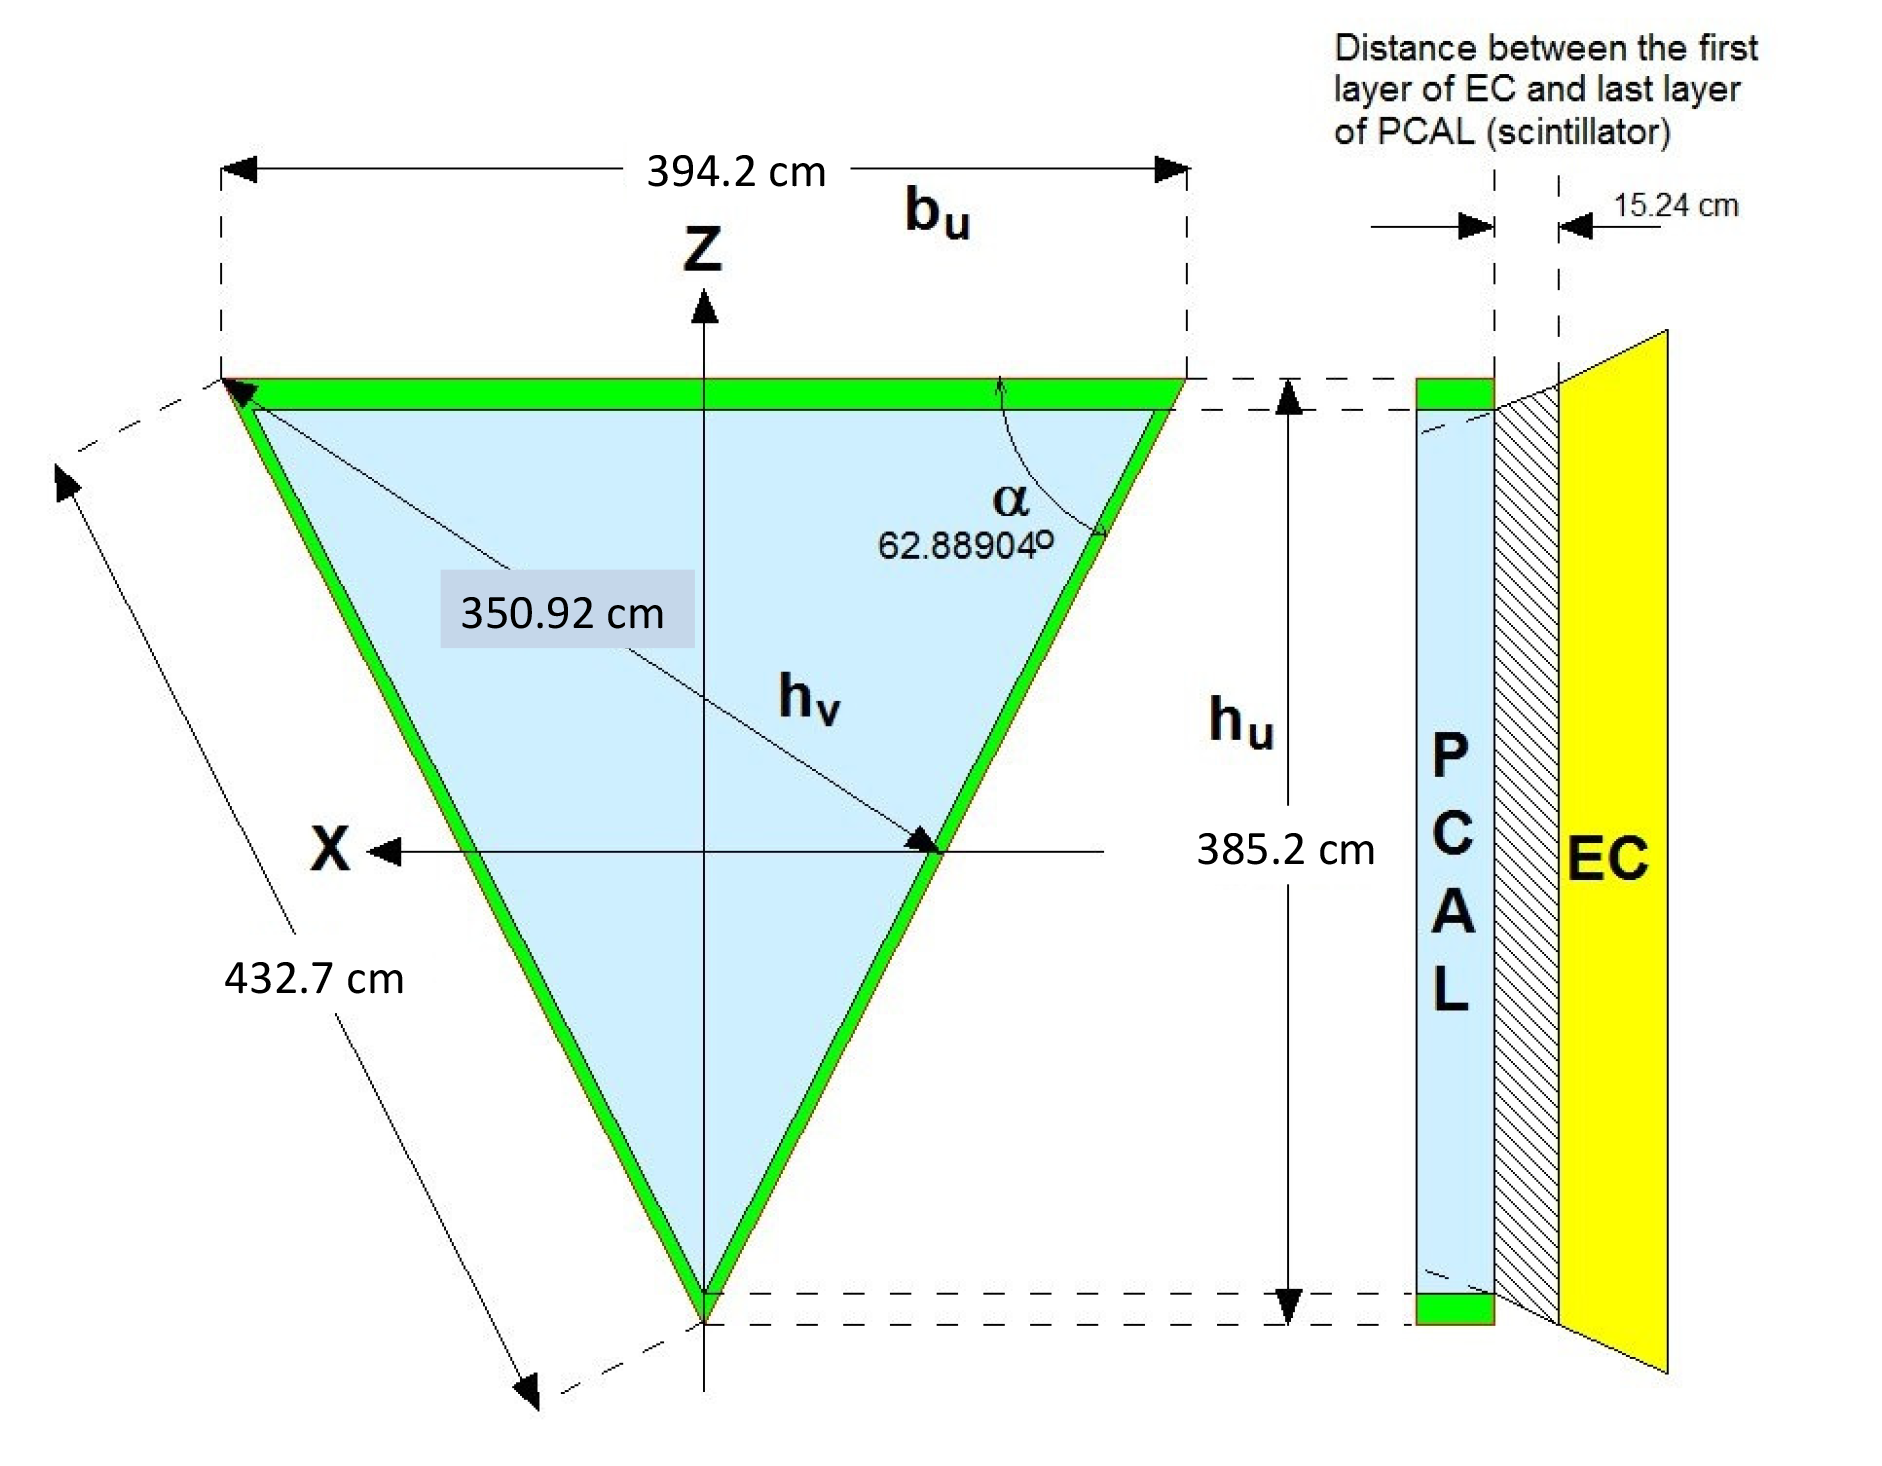
\includegraphics[width= 6in, keepaspectratio = true]{Pcal_geom_fig1}
    \caption{This diagram demonstrates the dimensions of the PCAL unit. This figure has been taken directly from the PCAL geometry note\cite{bib:geomnote}.}
    \label{fig:geomfig1}
\end{figure}

The PCAL box encapsulates layers of scintillator strips and lead sheets. 
Between each lead sheet there are three different orientations of scintillating strips. 
These orientations are described as the u, v, and w layers. 
Each layer is parallel with one side of the PCAL box. 
The sequencing of the lead sheet, u layer, v layer, and w layer is repeated five times within each sector of the PCAL unit. 
This results in fifteen layers of scintillator strips.
Each repeating layer signal is coupled to the same PMT, and  is not able to separate five different signals. 
A uvw view of the PCAL can be seen in figure \ref{fig:geomfig5}.


\begin{figure}[h]
    \centering
    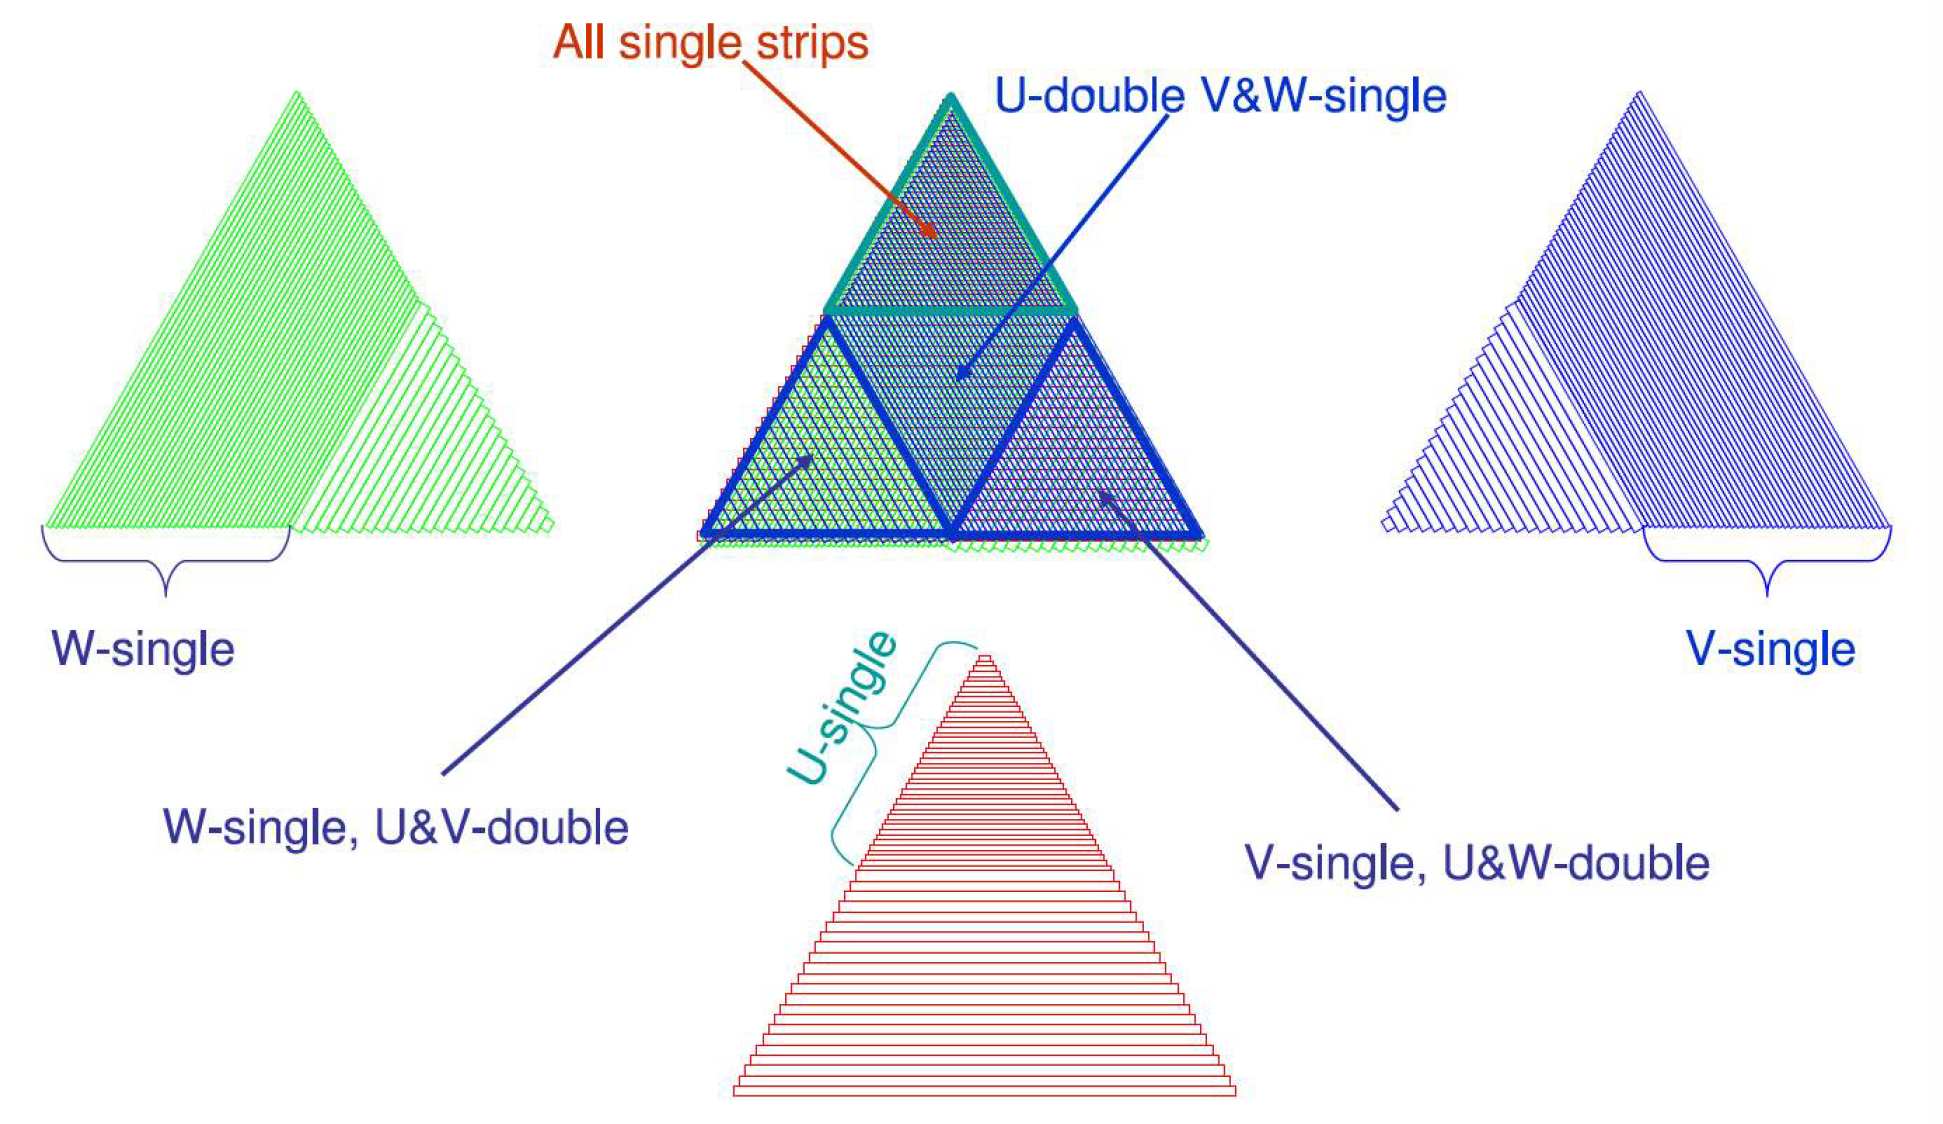
\includegraphics[width= 6in, keepaspectratio = true]{Pcal_geom_fig5}
    \caption{This is a schematic of how each orientation of scintillator is laid out. This figure is also taken directly from the PCAL geometry note\cite{bib:geomnote}.}
    \label{fig:geomfig5}
\end{figure}

There are 84 u strips, 77 v strips, and 77 w strips in each corresponding layer. 
The last 30 u strips are grouped into pairs to be readout to one PMT. 
The first 30 v and w strips are also grouped in pairs within their respective layer.
As a consequence there is better spatial resolution at low strip numbers in the u layer and at high numbers in the v and w layers. 
This pattern of scintillators can be seen in Figure \ref{fig:geomfig5}.







\section{Various Cuts}
The data used for calibration is from cosmic rays. These cosmic rays hit randomly throughout the PCAL unit. 
The distribution of these events although expected to be uniform, don't guarantee a good hit or detected signal in all three layers.
Moreover due to the strange pixel shapes and varying sizes different pixels have very different number of counts. 
An intitial skim was used to cut out events that would prevent a clean signal for calibration purposes.
Events were removed based on a multiplicity cut and a Dalitz condition.



\FloatBarrier
\subsection{Multiplicity Cut}
To ensure a more accurate calibration, a multiplicity cut was applied to collected data. 
The multiplicity cut removed any event that contained more than three PMT readouts (one in each layer). 
This reduces the number of cosmic ray events that are not relatively perpendicular to the face of the PCAL unit.
This is due to the fact that if a cosmic ray trajectory is not perpendicular to the PCAL face, it could clip multiple strips in one orientation (i.e. strip U30 and U31 both recieve a signal). Therefore by restricting the calibration to one perpendicular hit should, more well defined calibration constants could be determined. 
The accepted range of angles (different from perpendicular to the PCAL face) varies as a function of strip number and is not uniform in all directions.
This multiplicity cut also removes events where multiple cosmic rays hit the detector within the same time interval, due to possible firing of more PMTs. 



 \FloatBarrier
\subsection{Dalitz Cut} 
The Dalitz condition implies that if a point inside a triangle is chosen, no matter the location, the sum of the distances to each edge will be unchanged.
Rather than calculating each x and y point for every hit, distance as a function of strip width can be used to test this condition.
The relatively simple strip calculation can be computed by knowing the corresponding strip number to the triggered PMT combined with equations \ref{eq:udist}-\ref{eq:totaldist}.
This distance is empirically found to be two.
Preskimmed data demonstrating this distribution can be found at \url{https://clasweb.jlab.org/wiki/index.php/PCAL_Cosmic_Ray_Tests}. 
If this condition is not satisfied, then the hit recorded is most likely electronic noise, an indirect hit, or multiple cosmic ray hits recorded at once.

\begin{equation}
    dist(u) = \left\{
        \begin{array}{l l}
            u/84.0                       & \quad \text{if $u < 52$}\\
            (52.0 + (u - 52.0)\times2.0)/84.0 & \quad \text{if $u \geq 52$}
        \end{array} \right.{}
         \label{eq:udist}
\end{equation}

\begin{equation}
    dist(v) = \left\{
        \begin{array}{l l}
            2.0 \times v/77.0;                       & \quad \text{if $v < 15$}\\
            (30.0 + (v - 15.0))/77.0                 & \quad \text{if $v \geq 15$}
        \end{array} \right.{}
         \label{eq:vdist}
\end{equation}


\begin{equation}
    dist(w) = \left\{
        \begin{array}{l l}
            2.0 \times w/77.0;                       & \quad \text{if $w < 15$}\\
            (30.0 + (w - 15.0))/77.0                 & \quad \text{if $w \geq 15$}
        \end{array} \right.{}
         \label{eq:wdist}
\end{equation}


\begin{equation} 
    uvw = dist(u) +  dist(v) + dist(w)
    \label{eq:totaldist}
\end{equation}

\begin{figure}[h]
    \centering
    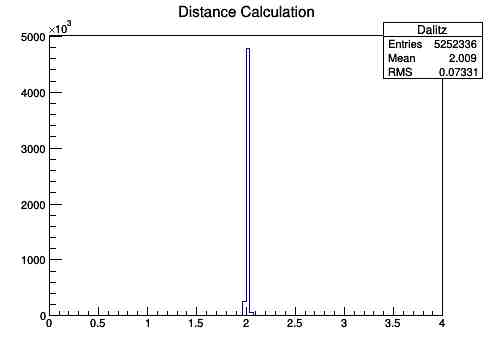
\includegraphics[height= 3in, keepaspectratio = true]{dalitz}
    \caption{Plotted is the resulting number ($uvw$) obtained from equation \ref{eq:totaldist} after the initial skim.}
    \label{fig:dalitz}
\end{figure} 


\FloatBarrier
\subsection{Unphysical Events}
\label{sec:unphysical}
An investigation into the types background was performed. 
Looking at an occupation number (events within a pixel), some recorded hits were unphysical if only one cosmic ray was considered to prompt the signal. 
Examples can be seen by Figures \ref{fig:unphysical} and \ref{fig:occupationnum}.

\begin{figure}[h]
    \centering
    \begin{subfigure}[h]{0.44\textwidth}
        \centering
        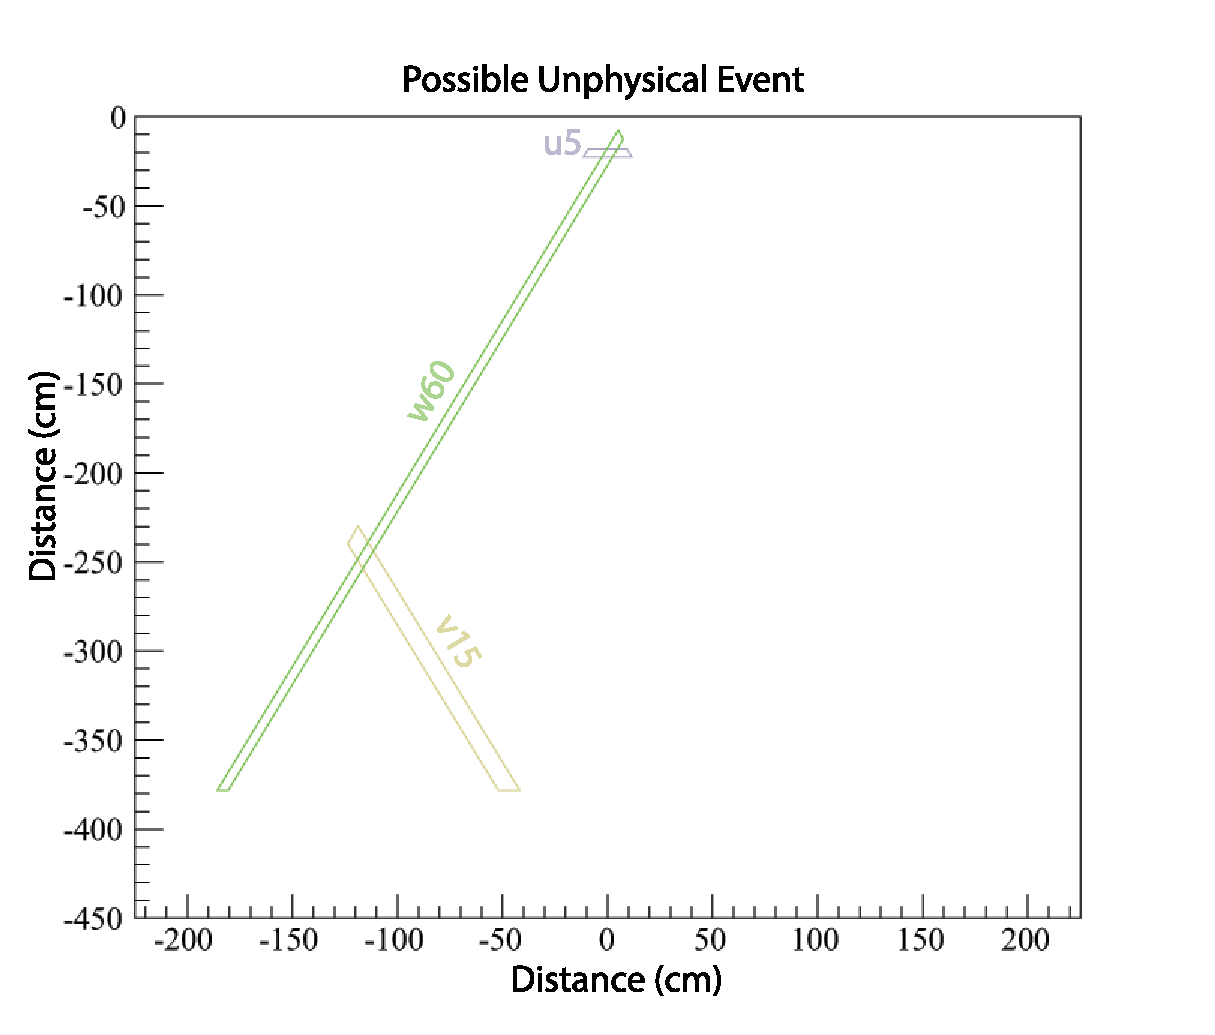
\includegraphics[width=\textwidth, keepaspectratio = true]{unphysical}
        \caption{Shown is one example of an event that would pass a multiplicity cut, but is clearly from either multiple rays or other noise.}
        \label{fig:unphysical}
    \end{subfigure}
    ~
    \begin{subfigure}[h]{0.44\textwidth}
        \centering
        \includegraphics[width=\textwidth, keepaspectratio = true]{pixelmap}
        \caption{Shown is a rough outline of the scintillator mapping created with minimal input.}
        \label{fig:pixelmap}
    \end{subfigure}
    \caption{Rough outline of the PCAL system.}
    \label{fig:pixelexplain}
\end{figure}

\begin{figure}[h]
\centering
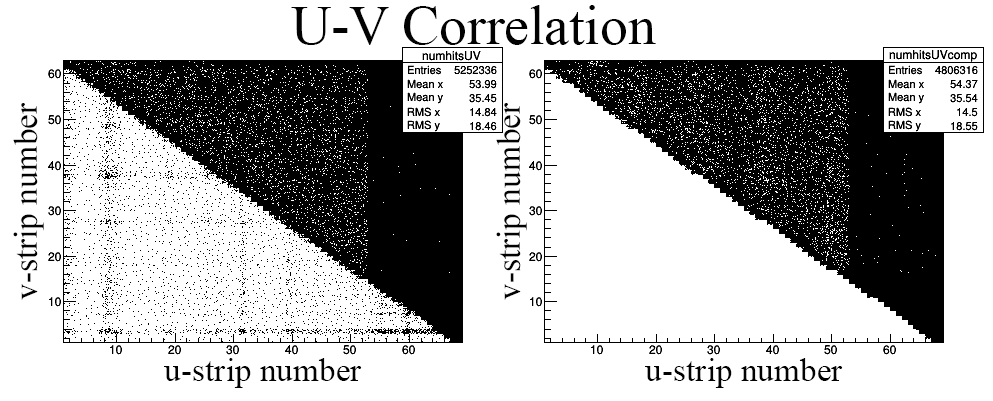
\includegraphics[width= 6in, keepaspectratio = true]{occupationnum}
\caption{The left histogram shows the u and v strip correlation after both the multiplicity and dalitz cuts were applied. The right histogram shows the u and v strip correlation after rejecting all unphysical background.}
\label{fig:occupationnum}
\end{figure}


The unphysical events can be spotted easily because low u and low v strip numbers should never correlate to just one incident cosmic ray.
To investigate in more detail, a program outlining the PCAL detector by strip number was generated.
This was generated using $\alpha$, $\beta$, number of strips, and strip width ($w$) as defined by Figure \ref{fig:stripwidth}. This outline or pixel mapping can be seen in Figure \ref{fig:pixelmap}.
This ideal outline of the system was then used in combination with a random number generator to verify which strip numbers could correlate to a physical perpendicular trajectory through the system.
These correlation numbers were then stored in tables and recalled in the analysis. Neighboring pixels in all directions were also marked as valid to account for uncertainty in the calculations and given numbers. 
Removing any event that did not end up in correlated PMTs results in no obvious unphysical signals as seen in figure \ref{fig:occupationnum}. 
However, looking at the signal distribution an exponential background still appears. This demonstrates that either different cuts and/or a very good fitting routine needs to be put in place.



\FloatBarrier


\section{Fit to ADC Output}
Although in general a three layer correlated pixel can be odd shaped, a two layer correlation can be straight forward. This two layer correlation creates trapezoidal bins formed by the overlap of two different strip orientations.\footnote{All of the studies in this section were primarily focused on the u strip attenuations, rather than the v/w strips.}
An example of one of these trapezoids outlined in black can be seen in figure \ref{fig:stripwidth}. 
Each one of these trapezoids should have a ADC readout value.
The width of this physical bin can be found by

\begin{equation}
    s = \frac{w}{\sin{\alpha}}
    \label{eq:s}
\end{equation}
or
\begin{equation}
    s = \frac{w}{\cos{\beta}},
\end{equation}
where $w$ is a single scintillator strip width ($\approx 4.5$cm).
Statistically one might expect some sort of peak describing the distribution of values. 
The centroid of this distribution is used as a data point at that center of that physical bin.

\begin{figure}[h]
\centering
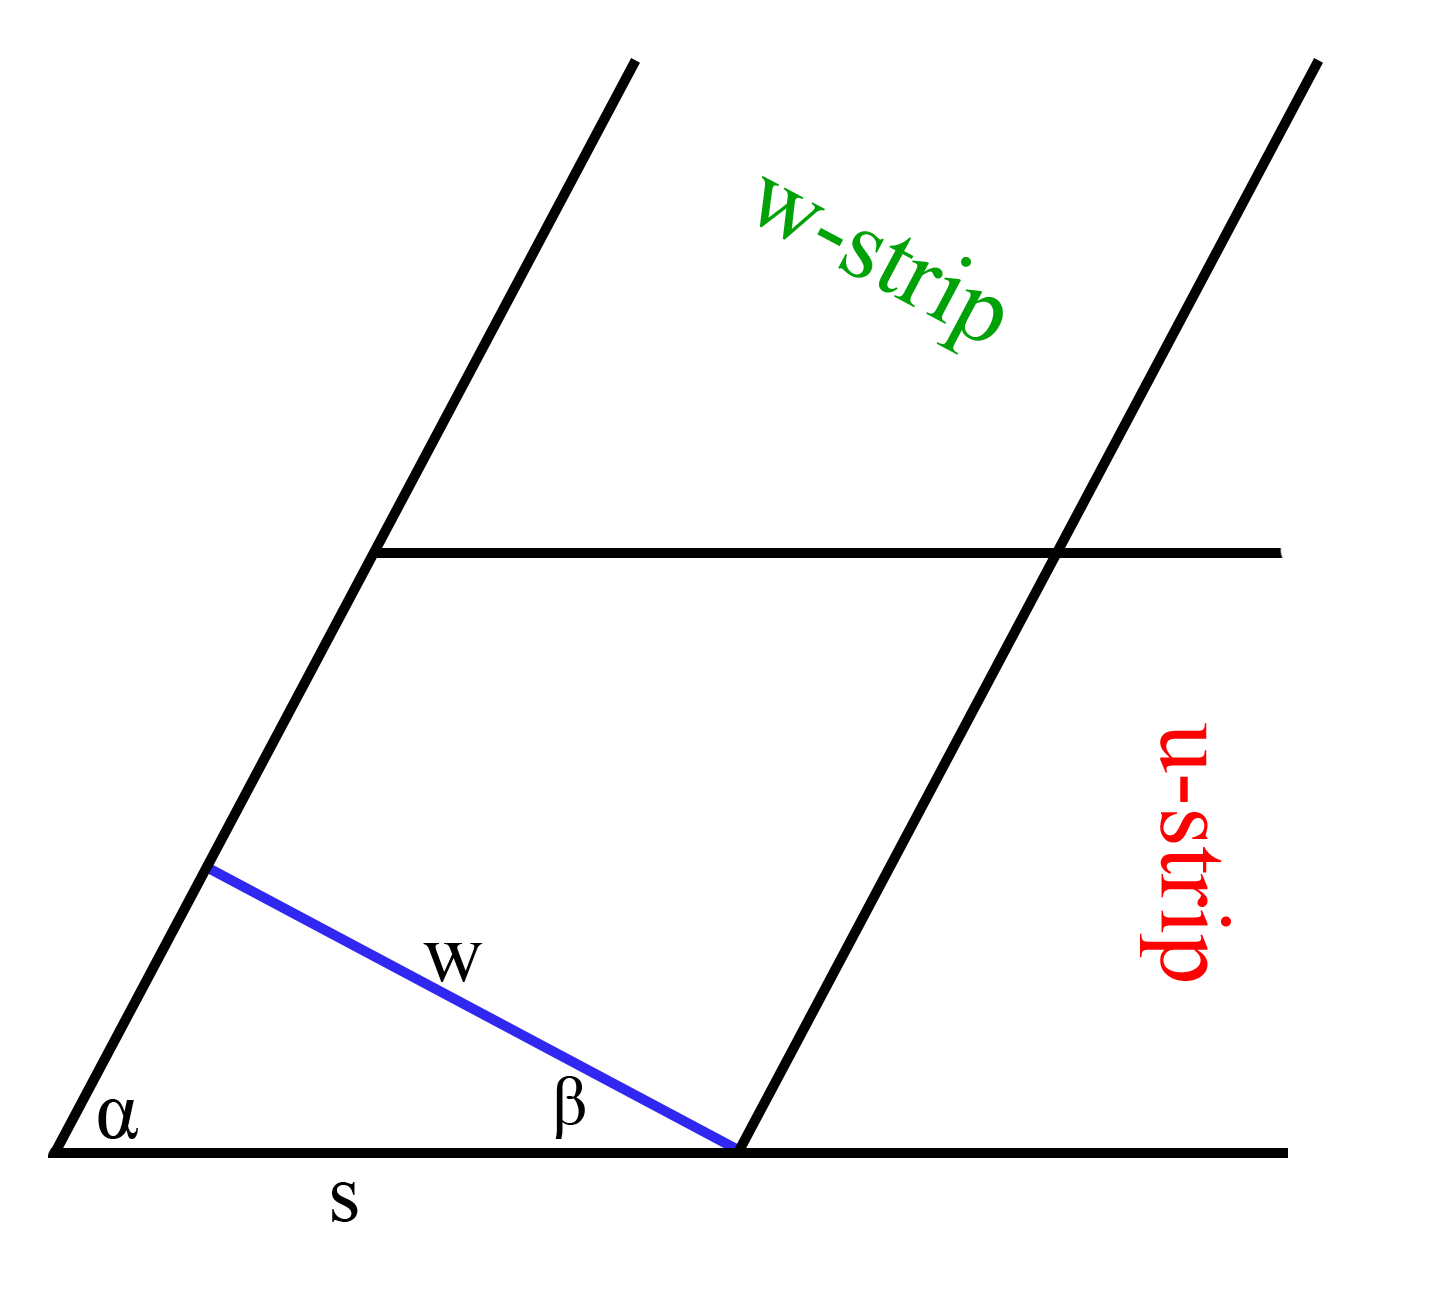
\includegraphics[width= 3in, keepaspectratio = true]{stripwidth}
\caption{Shown is an outline of a generic intersection of a u and w strip. The distance between the trapezoidal area and the PCAL edge can be represented by a linear function of $s$.}
\label{fig:stripwidth}
\end{figure}

\FloatBarrier
\subsection{Signal Shape}
The desired outcome is to approximate the signal by a simple function, for instance a Gaussian function.
Upon investigation the integrated ADC values appear to be a combination of a Gaussian and exponential fits.

\begin{figure}[h]
    \centering
    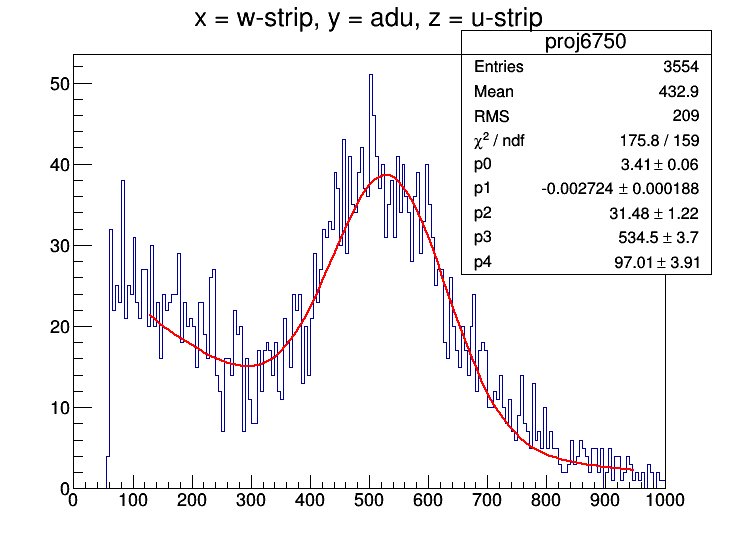
\includegraphics[width= 4in, keepaspectratio = true]{distribution}
    \caption{Shown is an example of the distribution of the ADC readout from one u/w trapezoidal bin (specifically the logical numbers u =67, w=50). The red line is a fit to an exponential combined with a Gaussian distribution.}
    \label{fig:distribution}
\end{figure}

This type of background can be seen for every physical two layered bin along any strip.

\begin{figure}[h]
    \centering
    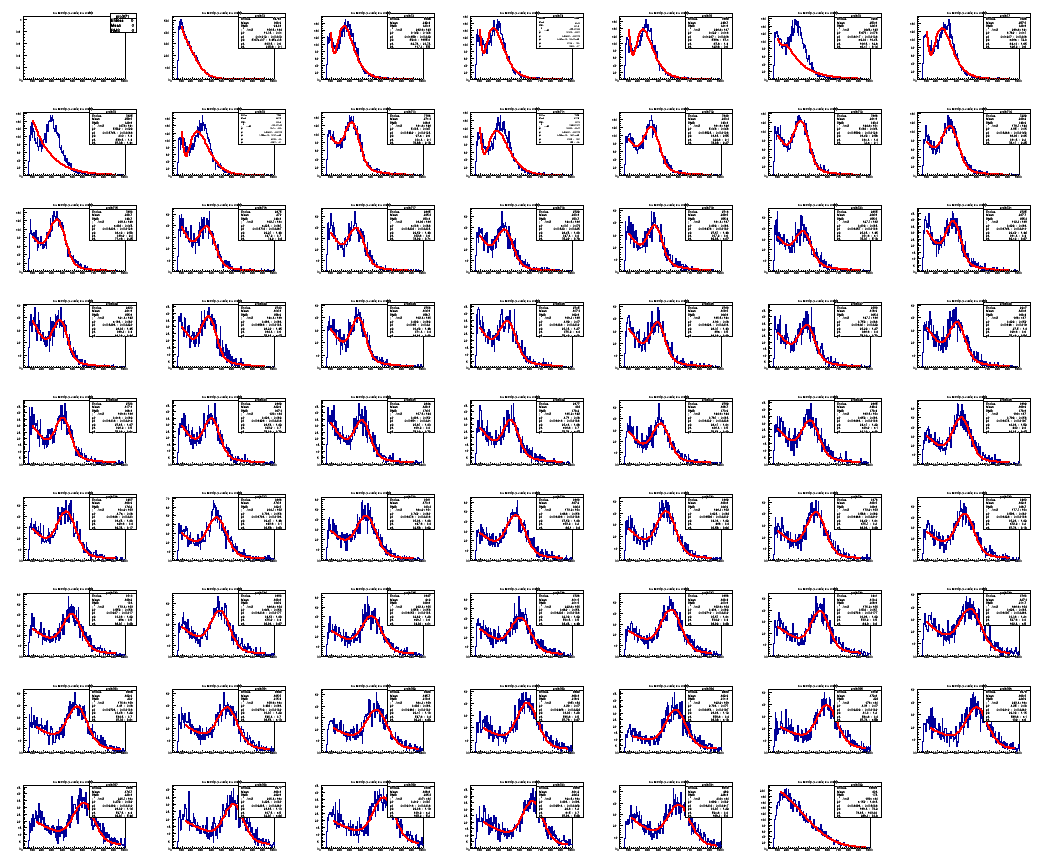
\includegraphics[width= 6in, keepaspectratio = true]{allstrip67}
    \caption{Shown is an example of all the distributions of the ADC readout from the 67th logical u strip.}
    \label{fig:allstrip67}
\end{figure}


\FloatBarrier
\subsubsection{Fit function}
Upon initial inspection the distribution is fit to an exponential and a Gaussian. 
The exponential is background/noise in most cases, whereas the Gaussian represents near perpendicular cosmic ray hits. 
The centroid of the Gaussian is extracted and determined to be the primary light intensity in that trapezoidal bin.

This plan works well for most interior physical bins. However, after looking at the strips corresponding to the edges of the PCAL unit, it is realized this can't be all that is done. Two possible improvements are utilized to better extend the calibration to the outer edges.

\begin{enumerate}
    \item Cut on each fit Gaussian signal. \\
        Using the fact that each bin in one scintillating strip corresponds to the other two, a cut on one affects the others. By making an iteration over all events a three sigma cut can be placed on each signal. This reduces the exponential background. This improves the fits to some of the edges.
    \item Cut on the overall energy deposited. \\
        Assuming that the signal is from the same cosmic ray and if that event doesn't participate in corner clipping, then the event should deposit the same amount of energy into each layer. After cutting on the original signal and fitting attenuation curves, individual gains can be approximated. Using the emperically found gains, a cut on the sum of ADC signals can be performed. This also helps the extend good fits to the edges of the pcal unit. This is the case due to the fact that two intersecting medium range strips (other layers) set limits on the possible events on the outer most strips. By improveing the outer most strips, they can be used to set limits on the overlapping shorter strips.  
\end{enumerate}

\FloatBarrier
\subsection{Iteration Process}
An iteration process was employed to improve the signal extraction. This process cuts events on ADC values determined by either the signal fits or by attenuation fits and then repeats. This allows for a converging result because each cut on one layer affects the other two. Therefore the raw signal fit keeps improving as the attenuation fit and gains improve. To illustrate how the process works, each iteration described in this section will describe cuts used when plotting the raw signal. After the cuts are describe an illustration of the fit to the signals will be shown with a diverse sampling (as diverse as six options gets). Next an attenuation fit over six of the strips will be shown. This shows how the multiple cuts affect each attenuation fits as a function of strip number. 

\clearpage
\FloatBarrier
\subsubsection{Pass 0}
\begin{itemize}
    \item Multiplicity Cut: Only events where one PMT fired for each strip were allowed.
    \item Dalitz Cut: An empircal distance sum was used to remove events that don't fall into this range determined by Equation \ref{eq:totaldist}.
    \item Valid hit or near neighbor hit: Using generated events on a calculated skeleton of the pcal, each pixel was determined to be valid or not. Extra uncertainty was allowed by also marking nearest neighboring pixels.
\end{itemize}

\begin{figure}[h]
    \centering
    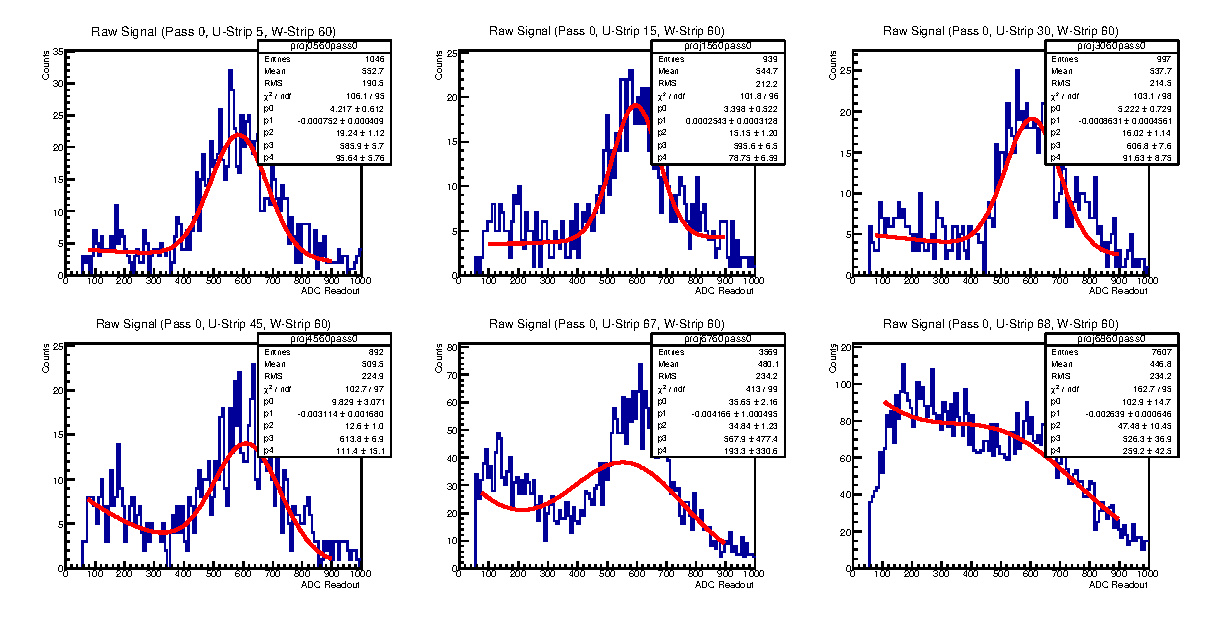
\includegraphics[height= 2.75in, keepaspectratio = true]{pass0}
    \caption{Shown is the ADC signal corresponding to signals from multiple u-strips (5, 15, 30, 45, 67, and 68) and a projection of the w60 strip.}
    \label{fig:pass0}
\end{figure}

\begin{figure}[h]
    \centering
    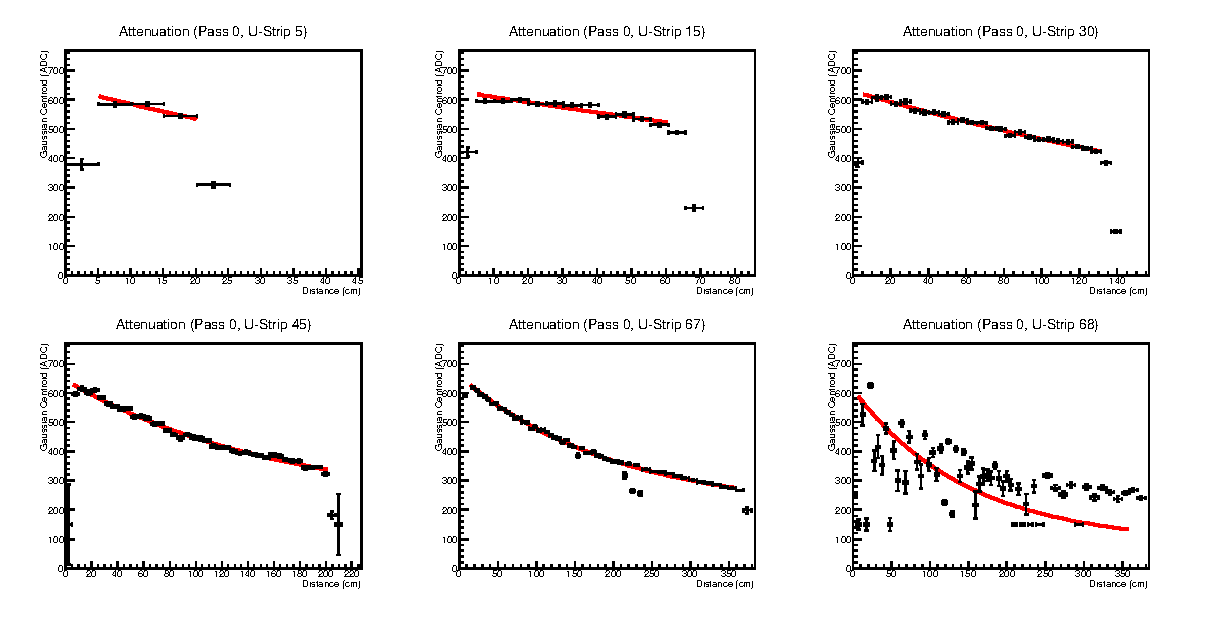
\includegraphics[height= 2.75in, keepaspectratio = true]{atpass0}
    \caption{Shown is the overall attenuation fits to the selected u-strips (5, 15, 30, 45, 67, and 68).}
    \label{fig:atpass0}
\end{figure}


\clearpage
\FloatBarrier
\subsubsection{Pass 1}
\begin{itemize}
    \item Multiplicity Cut: Only events where one PMT fired for each strip were allowed.
    \item Dalitz Cut: An empircal distance sum was used to remove events that don't fall into this range determined by Equation \ref{eq:totaldist}.
    \item Valid hit or near neighbor hit: Using generated events on a calculated skeleton of the pcal, each pixel was determined to be valid or not. Extra uncertainty was allowed by also marking nearest neighboring pixels.
    \item 3$\sigma$ Cut on Signal: Each signal was fit to a Gaussian and exponential in pass 0. The parameter $\sigma$ from the Gaussian fit was used to cut out the events that did not lie within this function.
\end{itemize}


\begin{figure}[h]
    \centering
    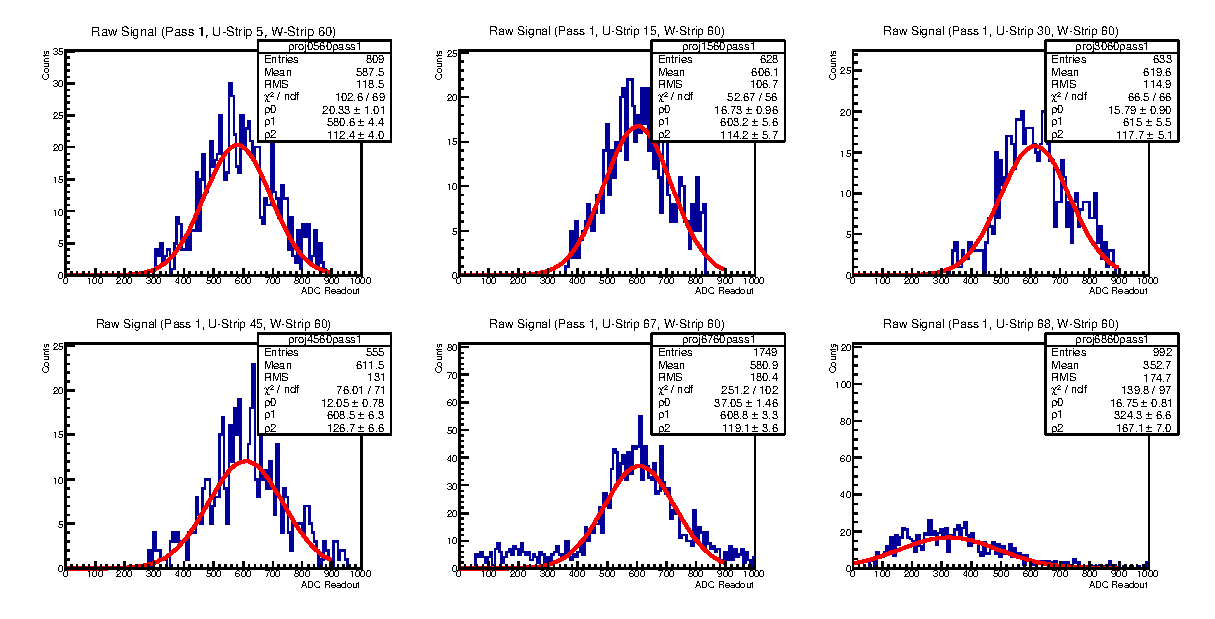
\includegraphics[height= 2.75in, keepaspectratio = true]{pass1}
    \caption{Shown is the ADC signal corresponding to signals from multiple u-strips (5, 15, 30, 45, 67, and 68) and a projection of the w60 strip.}
    \label{fig:pass1}
\end{figure}

\begin{figure}[h]
    \centering
    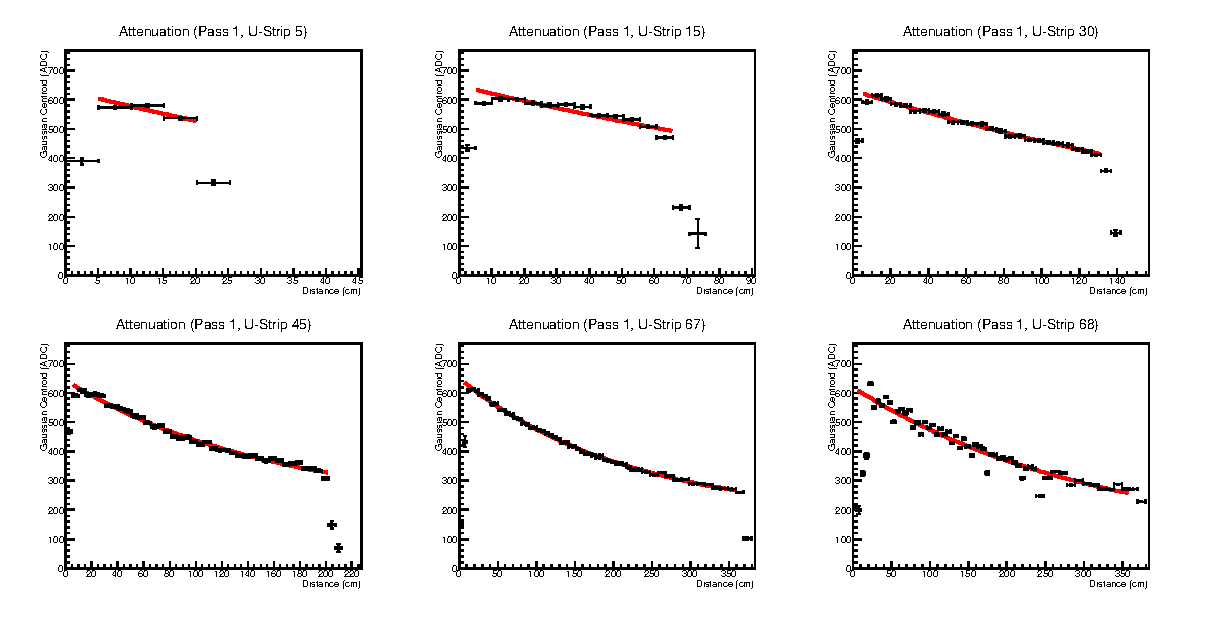
\includegraphics[height= 2.75in, keepaspectratio = true]{atpass1}
    \caption{Shown is the overall attenuation fits to the selected u-strips (5, 15, 30, 45, 67, and 68).}
    \label{fig:atpass1}
\end{figure}



\clearpage
\FloatBarrier
\subsubsection{Pass 2}
\begin{itemize}
    \item Multiplicity Cut: Only events where one PMT fired for each strip were allowed.
    \item Dalitz Cut: An empircal distance sum was used to remove events that don't fall into this range determined by Equation \ref{eq:totaldist}.
    \item Valid hit or near neighbor hit: Using generated events on a calculated skeleton of the pcal, each pixel was determined to be valid or not. Extra uncertainty was allowed by also marking nearest neighboring pixels.
    \item Cut on Attenuation Fits: When the signals where the Gaussian centroid from pass 1 were outside an ADC value of $\pm50$ from the attenuation fit, the obtained $\sigma$ was ignored and a new cut about the attenuation fit was employed. If the centroid was close to ADC value from the attenuation fit a 2$\sigma$ cut was used to remove extra background.
\end{itemize}


\begin{figure}[h]
    \centering
    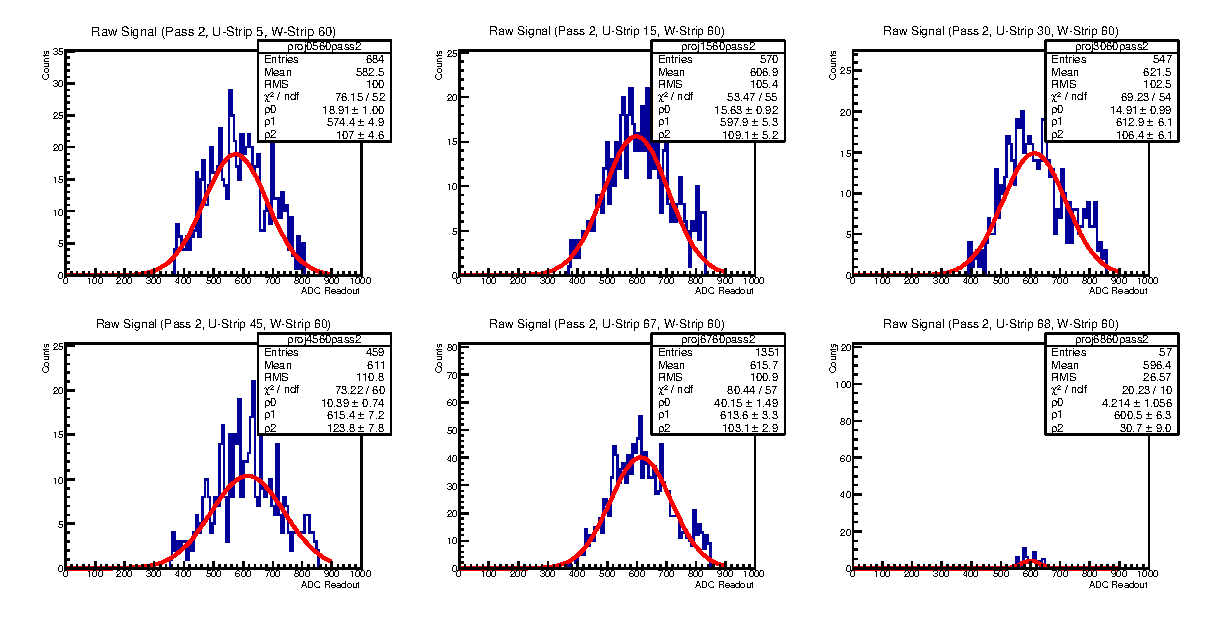
\includegraphics[height= 2.75in, keepaspectratio = true]{pass2}
    \caption{Shown is the ADC signal corresponding to signals from multiple u-strips (5, 15, 30, 45, 67, and 68) and a projection of the w60 strip.}
    \label{fig:pass2}
\end{figure}

\begin{figure}[h]
    \centering
    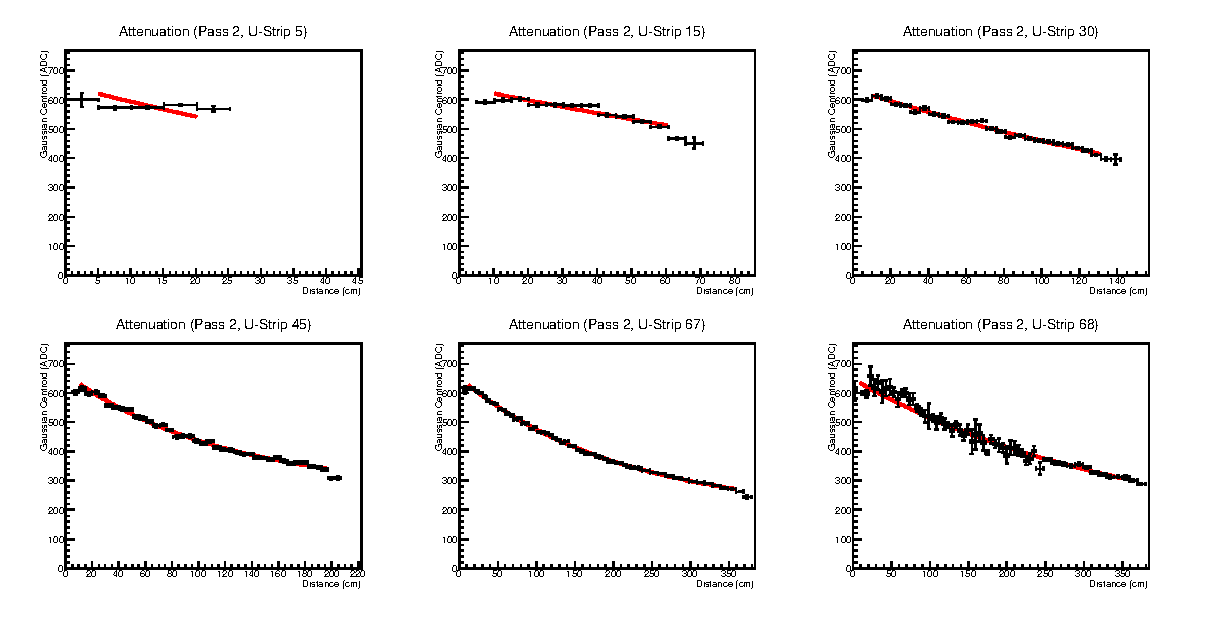
\includegraphics[height= 2.75in, keepaspectratio = true]{atpass2}
    \caption{Shown is the overall attenuation fits to the selected u-strips (5, 15, 30, 45, 67, and 68).}
    \label{fig:atpass2}
\end{figure}



\clearpage
\FloatBarrier
\subsubsection{Pass 3}
\begin{itemize}
    \item Multiplicity Cut: Only events where one PMT fired for each strip were allowed.
    \item Dalitz Cut: An empircal distance sum was used to remove events that don't fall into this range determined by Equation \ref{eq:totaldist}.
    \item Valid hit: Using generated events on a calculated skeleton of the pcal, each pixel was determined to be valid or not.
    \item 3$\sigma$ Cut on Signal: Each signal was fit to a Gaussian in pass 2. The parameter $\sigma$ from the Gaussian fit was used to cut out the events that did not lie within this function.
    \item Attenuation Corrected Intensity Cut: The ADC value measured was corrected with the attenuation curves obtained from pass 2. The corrected value was summed over each layer. A cut on this intensity was placed generously from 1300 to 2700
\end{itemize}

\begin{figure}[h]
    \centering
    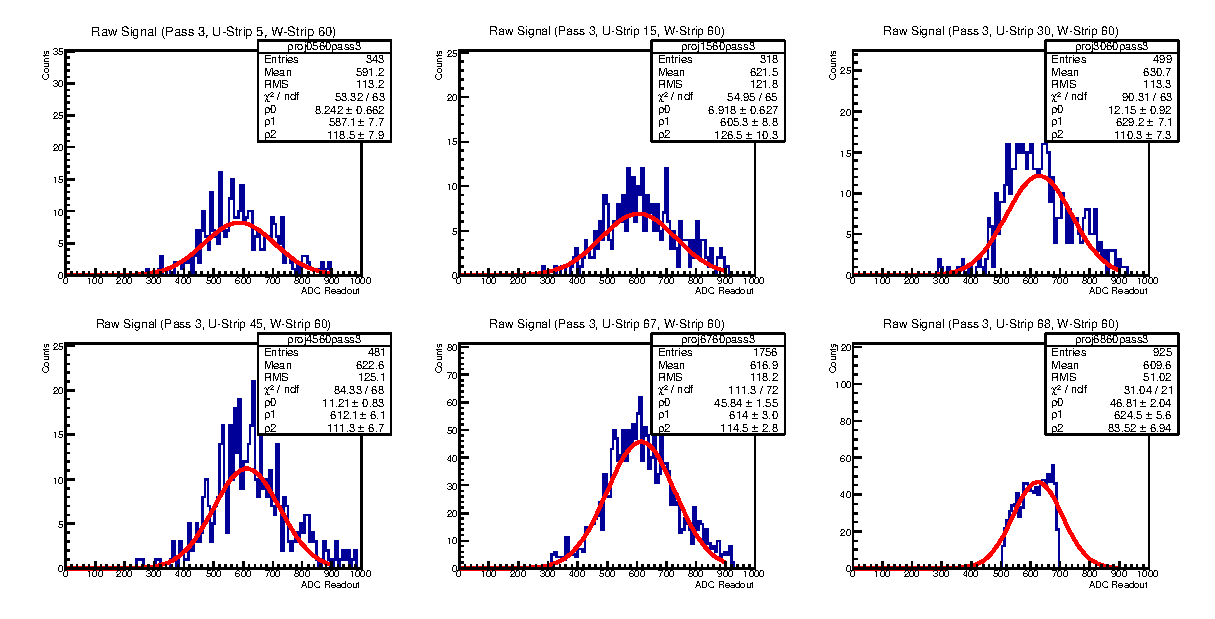
\includegraphics[height= 2.75in, keepaspectratio = true]{pass3}
    \caption{Shown is the ADC signal corresponding to signals from multiple u-strips (5, 15, 30, 45, 67, and 68) and a projection of the w60 strip.}
    \label{fig:pass3}
\end{figure}

\begin{figure}[h]
    \centering
    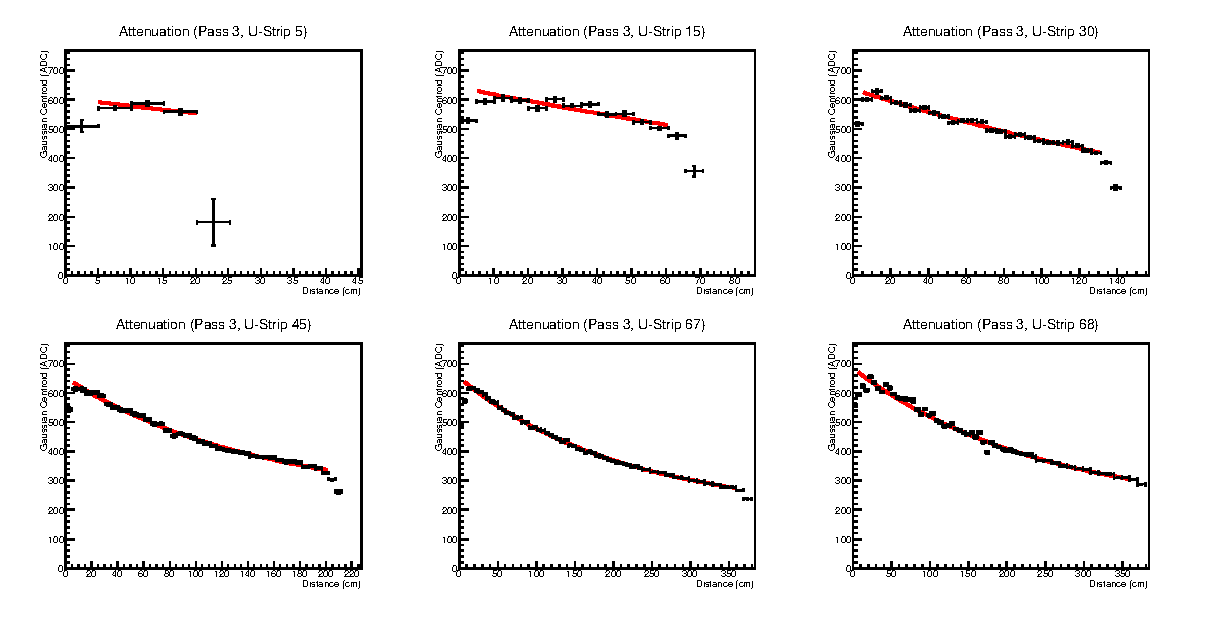
\includegraphics[height= 2.75in, keepaspectratio = true]{atpass3}
    \caption{Shown is the overall attenuation fits to the selected u-strips (5, 15, 30, 45, 67, and 68).}
    \label{fig:atpass3}
\end{figure}

\clearpage
\FloatBarrier
\subsubsection{Pass 4}
\begin{itemize}
    \item Multiplicity Cut: Only events where one PMT fired for each strip were allowed.
    \item Dalitz Cut: An empircal distance sum was used to remove events that don't fall into this range determined by Equation \ref{eq:totaldist}.
    \item Valid hit: Using generated events on a calculated skeleton of the pcal, each pixel was determined to be valid or not.
    \item 3$\sigma$ Cut on Signal: Each signal was fit to a Gaussian in pass 2. The parameter $\sigma$ from the Gaussian fit was used to cut out the events that did not lie within this function.
    \item Attenuation Corrected Intensity Cut: The ADC value measured was corrected with the attenuation curves obtained from pass 2. The corrected value was summed over each layer. A cut on this intensity was placed generously from 1300 to 2700
\end{itemize}


\begin{figure}[h]
    \centering
    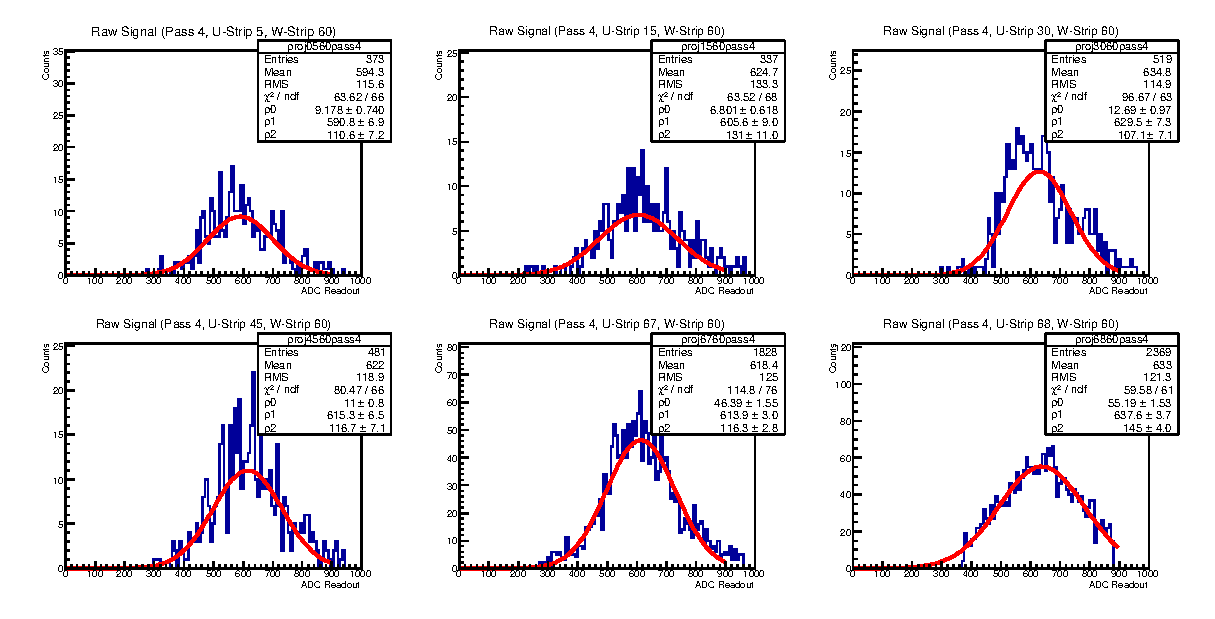
\includegraphics[height= 2.75in, keepaspectratio = true]{pass4}
    \caption{Shown is the ADC signal corresponding to signals from multiple u-strips (5, 15, 30, 45, 67, and 68) and a projection of the w60 strip.}
    \label{fig:pass4}
\end{figure}

\begin{figure}[h]
    \centering
    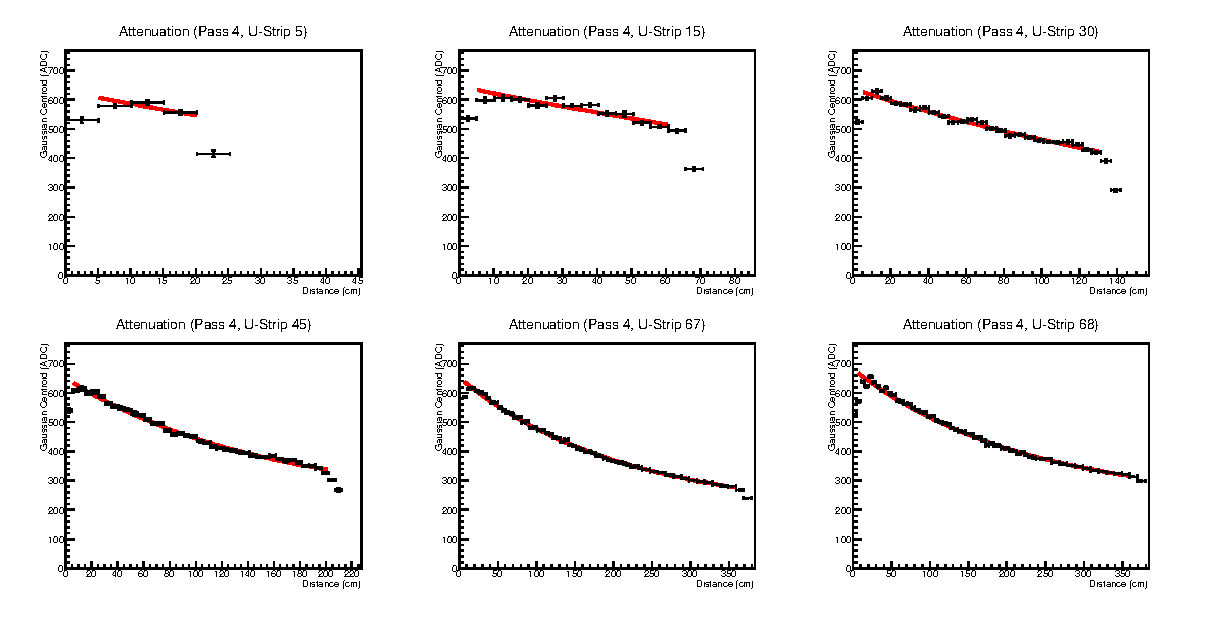
\includegraphics[height= 2.75in, keepaspectratio = true]{atpass4}
    \caption{Shown is the overall attenuation fits to the selected u-strips (5, 15, 30, 45, 67, and 68).}
    \label{fig:atpass4}
\end{figure}


\clearpage
\FloatBarrier
\subsubsection{Pass 5}
\begin{itemize}
    \item Multiplicity Cut: Only events where one PMT fired for each strip were allowed.
    \item Dalitz Cut: An empircal distance sum was used to remove events that don't fall into this range determined by Equation \ref{eq:totaldist}.
    \item Valid hit: Using generated events on a calculated skeleton of the pcal, each pixel was determined to be valid or not.
    \item 3$\sigma$ Cut on Signal: Each signal was fit to a Gaussian in pass 2. The parameter $\sigma$ from the Gaussian fit was used to cut out the events that did not lie within this function.
    \item Attenuation Corrected Intensity Cut: The ADC value measured was corrected with the attenuation curves obtained from pass 2. The corrected value was summed over each layer. A cut on this intensity was placed generously from 1300 to 2700
\end{itemize}
               
               


\begin{figure}[h]
    \centering
    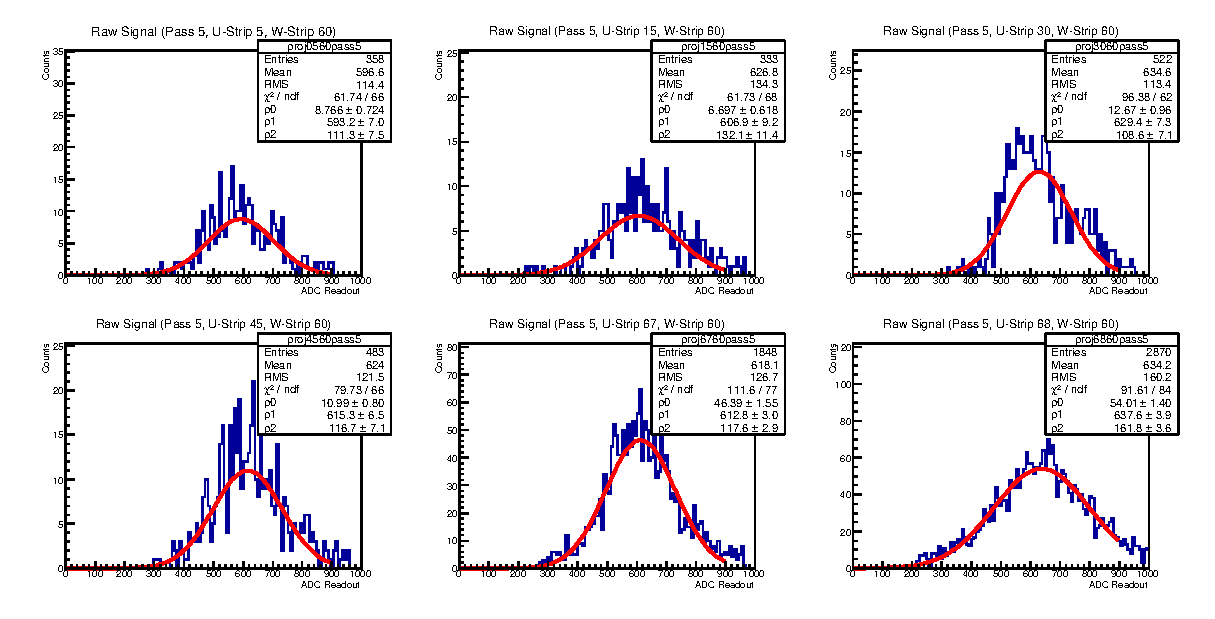
\includegraphics[height= 2.75in, keepaspectratio = true]{pass5}
    \caption{Shown is the ADC signal corresponding to signals from multiple u-strips (5, 15, 30, 45, 67, and 68) and a projection of the w60 strip.}
    \label{fig:pass5}
\end{figure}

\begin{figure}[h]
    \centering
    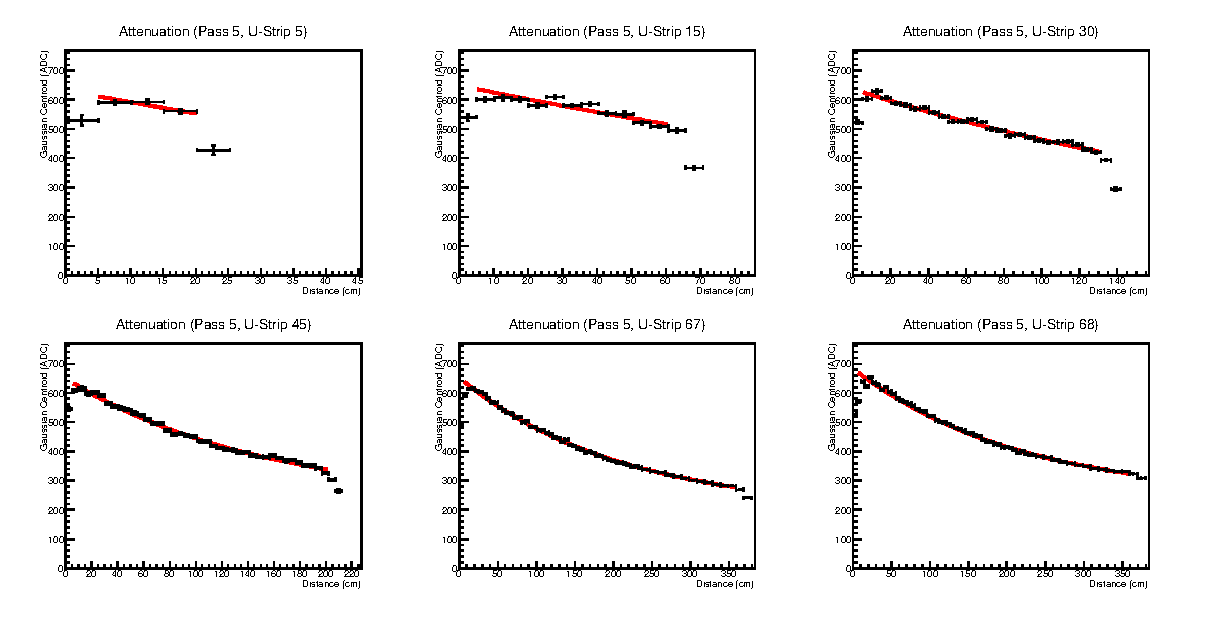
\includegraphics[height= 2.75in, keepaspectratio = true]{atpass5}
    \caption{Shown is the overall attenuation fits to the selected u-strips (5, 15, 30, 45, 67, and 68).}
    \label{fig:atpass5}
\end{figure}


\FloatBarrier


\begin{figure}[h]
    \centering
    \begin{subfigure}[h]{0.3\textwidth}
        \centering
        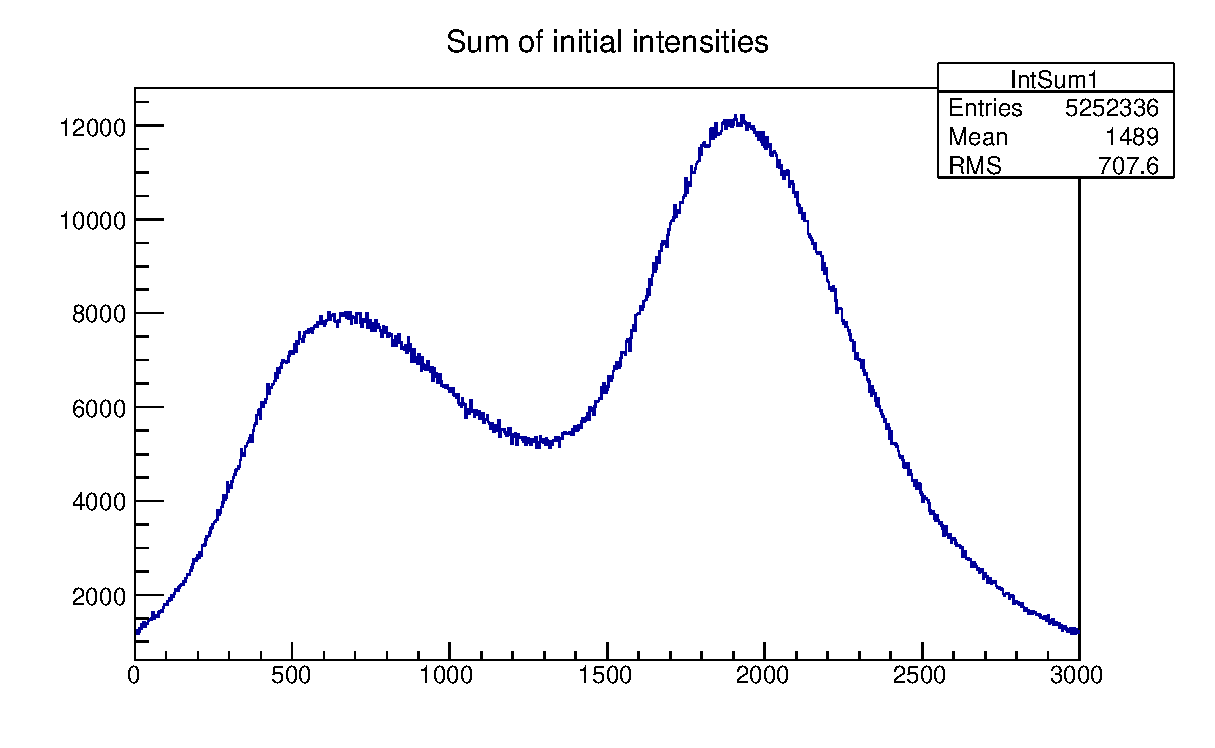
\includegraphics[width=\textwidth, keepaspectratio = true]{nocutsIsum}
        \caption{Sum of all initial intensities. No cuts.}
        \label{fig:nocutsIsum}
    \end{subfigure}
    ~
    \begin{subfigure}[h]{0.3\textwidth}
        \centering
        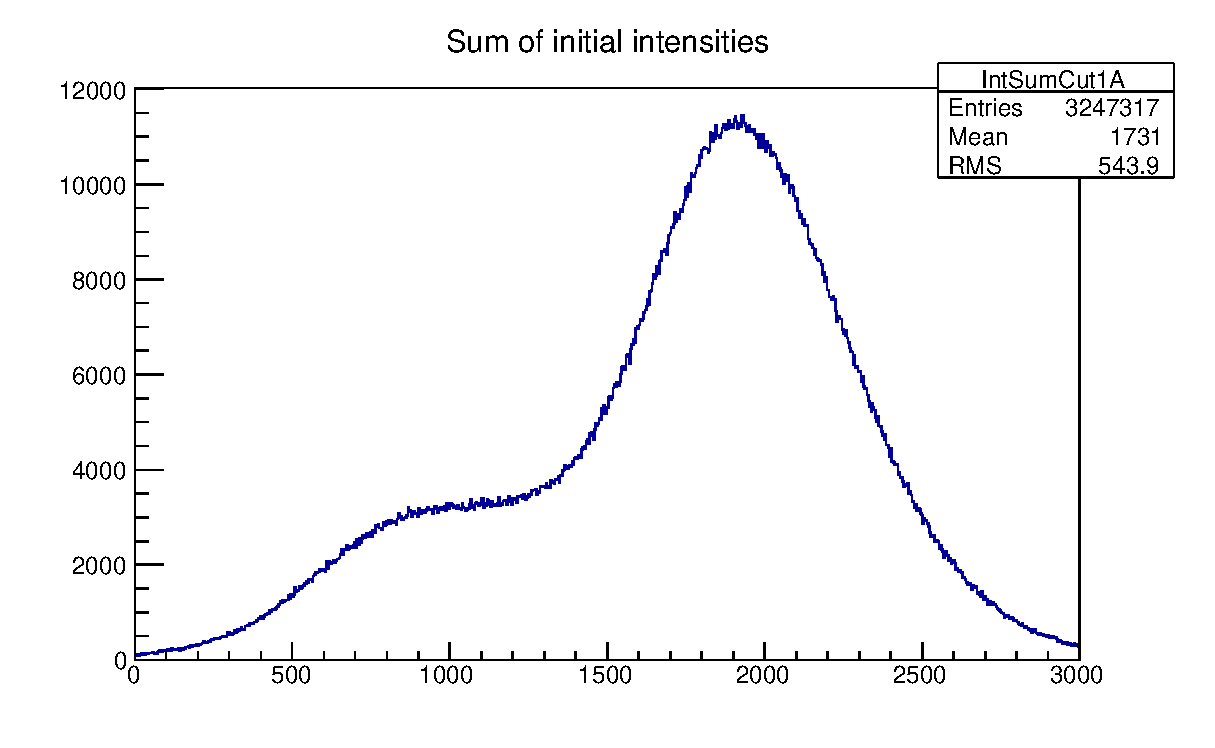
\includegraphics[width=\textwidth, keepaspectratio = true]{3sigcutIsum}
        \caption{Sum of all initial intensities. Three sigma Cut.}
        \label{fig:3sigcutIsum}
    \end{subfigure}
    ~
    \begin{subfigure}[h]{0.3\textwidth}
        \centering
        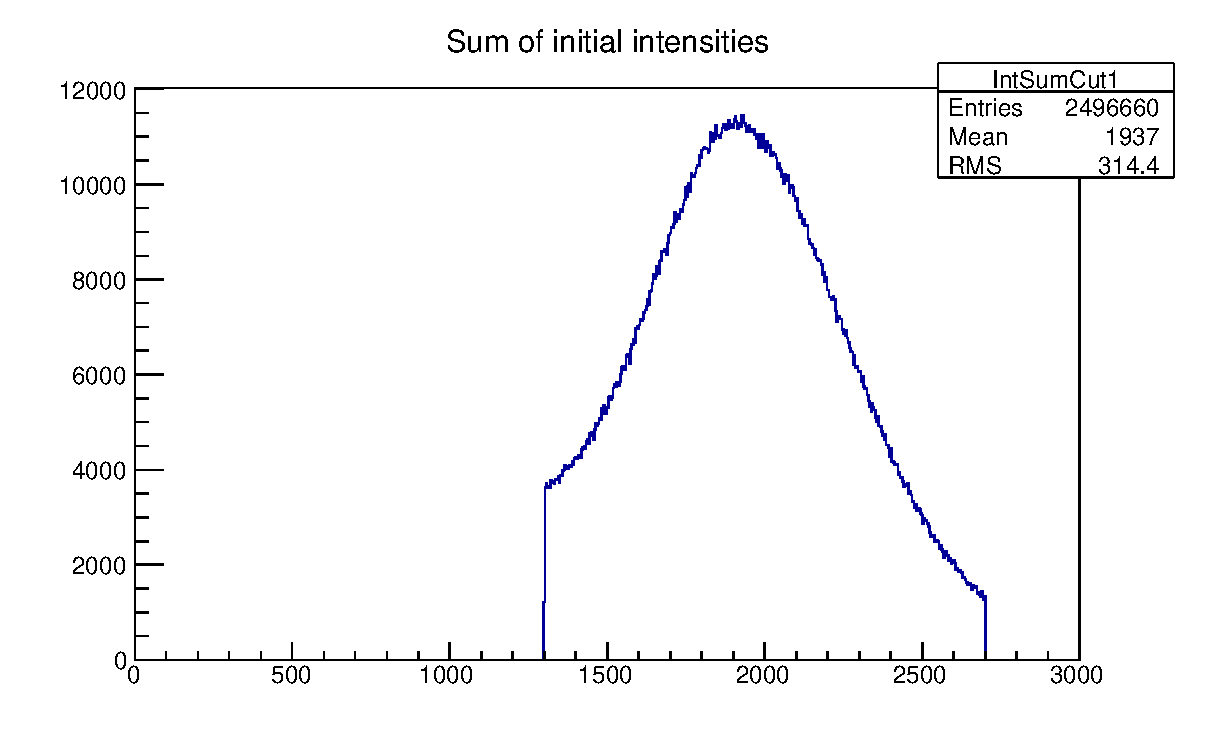
\includegraphics[width=\textwidth, keepaspectratio = true]{allcutsIsum}
        \caption{Sum of all initial intensities. Three sigma and sum Cut.}
        \label{fig:allcutsIsum}
    \end{subfigure}
    \caption{Sum of initial intensities should be near $650 \times 3 = 1950$ (after gain corrections).}
    \label{fig:intensities}
\end{figure}

\FloatBarrier
\subsection{Comparison of Fits}
Possibly the best evidence for needed cuts about each signal in an iterative process is seen by looking at the raw signal fits for a w strip with the possible u projections. These comparisons can be seen from pass 0 to pass 5 in Figures \ref{fig:w61sigfitpass0} and \ref{fig:w61sigfitpass5}. The difference between these signal tends to be cleaned up to a more Gaussian signal. By itself it is difficult to remove the backgound, but due to the correlating cuts on the u and v layers a reasonable output is produced.

\begin{figure}[h]
    \centering
    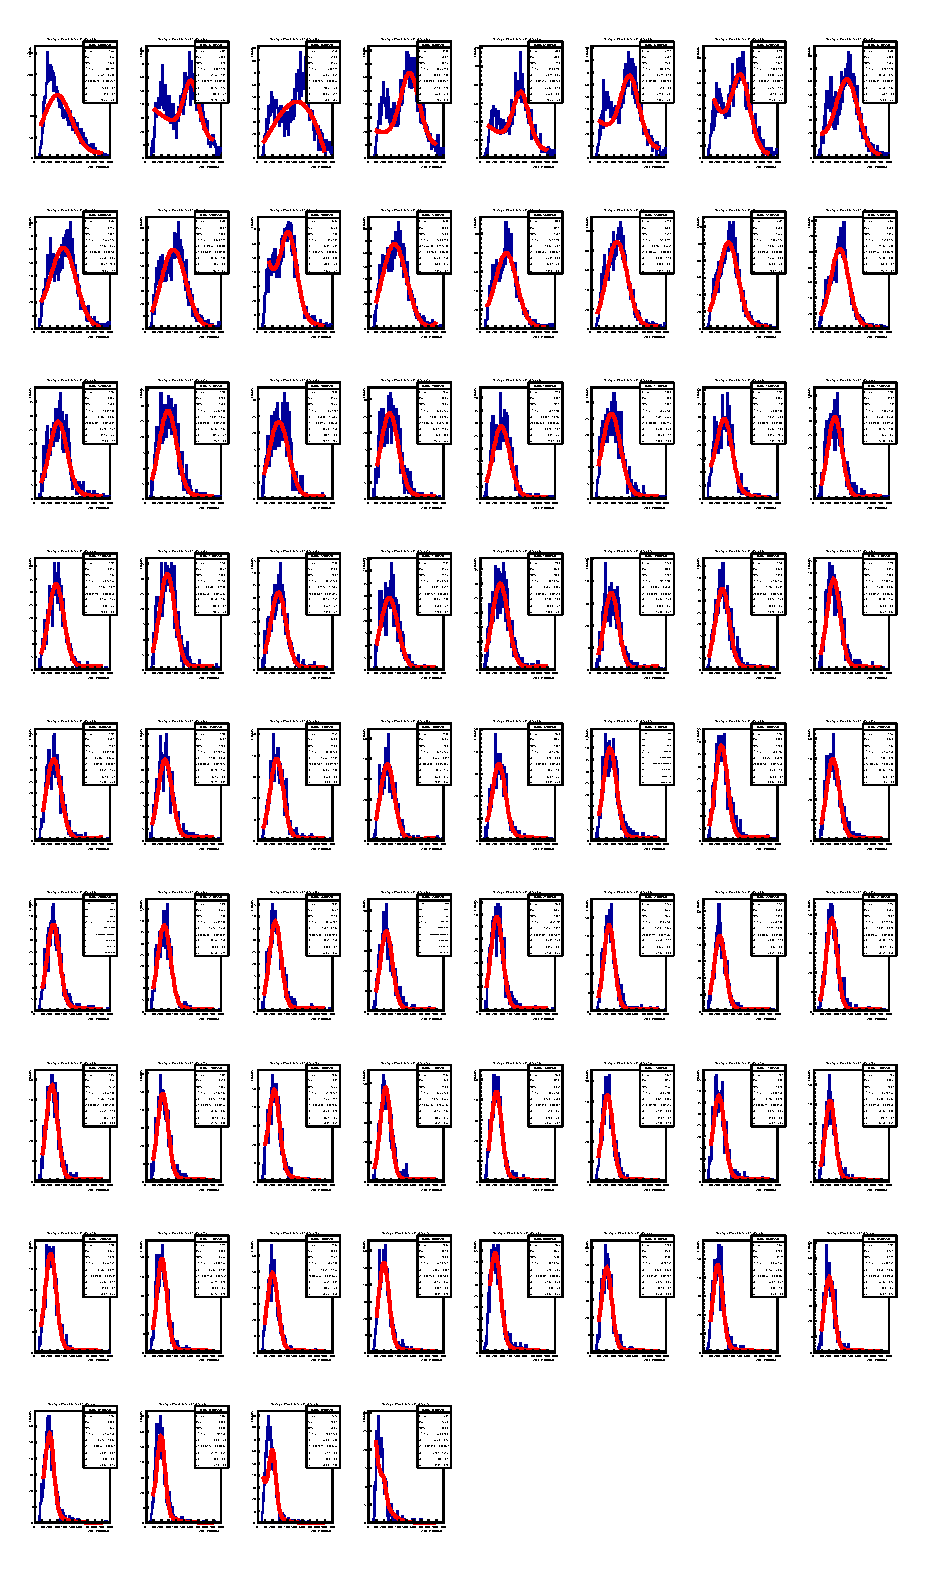
\includegraphics[width=\textwidth, height= 8in, keepaspectratio = true]{w61sigfitpass0}
    \caption{Shown is the ADC signal corresponding to signals from multiple u-strip projections of the w61 strip (pass0).}
    \label{fig:w61sigfitpass0}
\end{figure}

\begin{figure}[h]
    \centering
    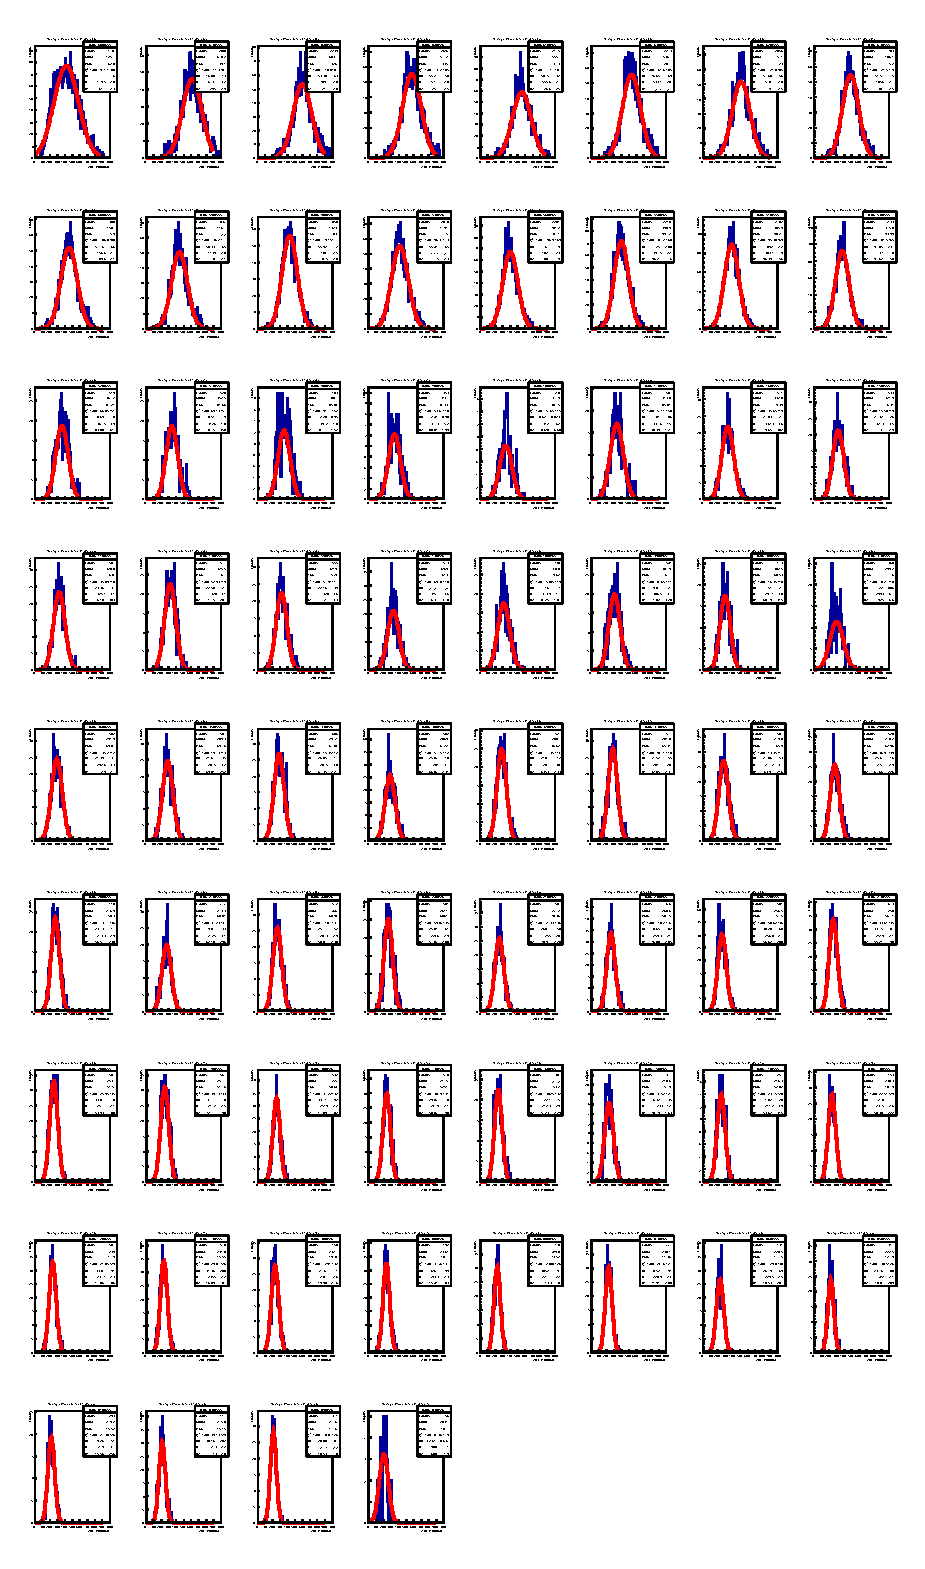
\includegraphics[width=\textwidth, height= 8in, keepaspectratio = true]{w61sigfitpass5}
    \caption{Shown is the ADC signal corresponding to signals from multiple u-strip projections of the w61 strip (pass5).}
    \label{fig:w61sigfitpass5}
\end{figure}


\FloatBarrier



\section{Light Attenuation}
Fits are done based on trapezoidal bins corresponding to strip number. 
The strip number is converted into distance by a process using equations \ref{eq:udist}-\ref{eq:wdist}, equation \ref{eq:s}, and an offset to have the distance quoted to the center of the physical bin. 
The exccess fiber lengths in theory could be added into the distance, but will only cause a shift in the fit.
The fiber lengths are taken from the PCAL geometry note \cite{bib:geomnote}. 
% and are listed in section \ref{sec:fiberlength}.
The Gaussian centroids can be found as a function of total distance from the edge of the PCAL unit.
This total distance is fit to an exponential form. 




\subsection{Strip Number vs Distance}
\FloatBarrier

The overlaid strip numbers convert directly into distance as seen by Figure \ref{fig:lowqualdist}

\begin{figure}[h]
\centering
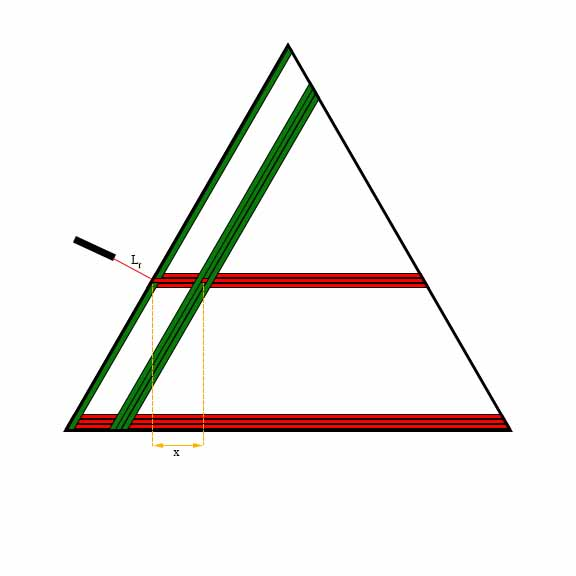
\includegraphics[height= 3in, keepaspectratio = true]{lowqualitydiagram}
\caption{A cartoon schematic of the pcal unit demonstrates the method to correct for the light attenuation.}
\label{fig:lowqualdist}
\end{figure}


%\FloatBarrier
%\subsection{Fiber Length}
%\label{sec:fiberlength}
%Fiber lengths for each individual strip can be found in the PCAL geometry note \cite{bib:geomnote}.
%These table have been recorded and added into the calibration. 



\FloatBarrier
\subsection{Fit Function}
\FloatBarrier
The fit function suggested in the geometry note is an  exponential (equation \ref{eq:exp}).
It is also suggested that here the distance, $L$, should include the distance from the end of the strip to the cosmic ray track, $L_{s}$, as well as the extra fiber length, $L_{f}$.
In other words $L = L_{s} + L_{f}$.
However to analyze the quality of fit $L_{f}$ can be treated as a constant and absorbed into the parameter $a$ in equation \ref{eq:exp}.

\begin{equation}
    I = e^{a + bL}
    \label{eq:exp}
\end{equation}

\begin{figure}[h]
    \centering
    \begin{subfigure}[h]{0.4\textwidth}
        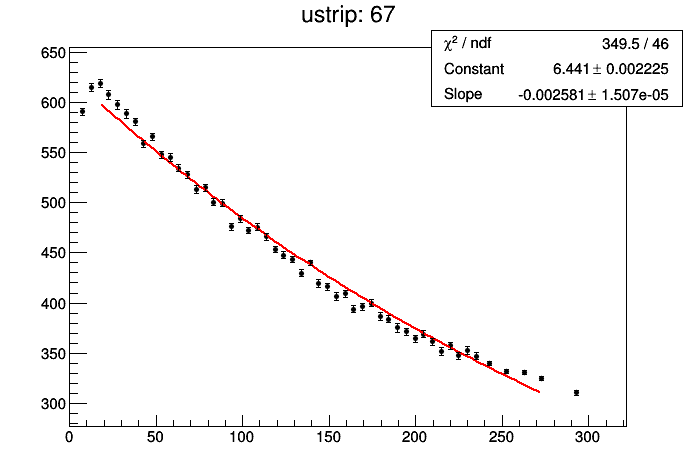
\includegraphics[width= \textwidth, keepaspectratio = true]{exponetial67}
        \caption{Shown is a fit with equation \ref{eq:exp}, where the y axis is the ADC value and the x axis is $L_{s}$.}
        \label{fig:exponential67}
    \end{subfigure}
    ~
    \begin{subfigure}[h]{0.4\textwidth}
        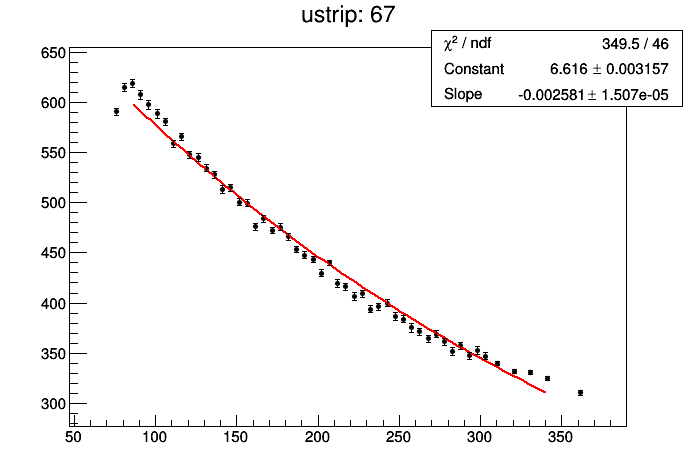
\includegraphics[width= \textwidth, keepaspectratio = true]{exponetialwfib67}
        \caption{Shown is a fit with equation \ref{eq:exp}, where the y axis is the ADC value and the x axis is $L_{s} + L_{f}$.}
        \label{fig:exponentialwfib67}
    \end{subfigure}
    \caption{Plotted is the fit of equation \ref{eq:exp}, where $L = L_{s}$ (a) and $L = L_{s} + L_{f}$ (b).}
    \label{fig:expfit}
\end{figure}

As seen by figure \ref{fig:expfit}, a single exponential may not be the best fit for the data.
One might suggest a fitting function similar to equation \ref{eq:try1}, in order to separate the fiber attenuation from the scintillator attenuation.
However this function again can reduce to equation \ref{eq:exp} because $L_{f}$ is a constant for each scintillator strip and is seen not to be a good fit.


\begin{equation}
    \begin{split}
        I &= a_{1}e^{b_{1}(L_{s} + L_{f})}e^{b_{2}L_{s}} \\
          &= a_{1}e^{b_{1}(L_{s} + L_{f}) + b_{2}L_{s}} \\
          &= a_{1}e^{(b_{1} + b_{2})L_{s} + b_{1}L_{f}} \\
          &= a_{1}e^{b_{1}L_{f}}e^{(b_{1} + b_{2})L_{s}} \\
          &= e^{a}e^{(b_{1} + b_{2})L_{s}} \\
          &= e^{a}e^{bL_{s}} \\
          &= e^{a + bL_{s}} \\
    \end{split}
    \label{eq:try1}
\end{equation}

\begin{comment}
\begin{equation}
    I(L_{s})= ae^{(b_{1} + b_{2})L_{s} + b_{1}L_{f}}
    \label{eq:try1mid}
\end{equation}

\FloatBarrier
\begin{figure}[h]
    \centering
    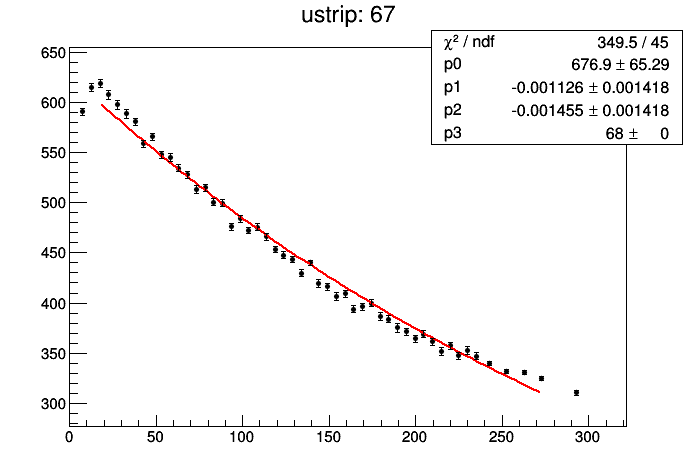
\includegraphics[width= 3in, keepaspectratio = true]{exponential67eq9}
    \caption{Plotted is the fit of equation \ref{eq:try1mid} as a function of $L_{s}$.}
    \label{fig:try1mid}
\end{figure}
\end{comment}
\FloatBarrier


Other functional forms that could represent the data should be similar to that of an exponential.
A couple of these forms include an exponential plus a constant or a sum of exponentials.
In both cases, some considerations have to be made on the domain of the function.
The sum of two exponentials was considered to have some portion of the attenuation in the fibers to be different than inside the scintillator. This does not get a better fit, and does not allow any more information to be extracted. Therefore the function used in fitting the attenuation was chosen to be an exponential with an added constant as seen by Equation \ref{eq:expplusconst}.

\begin{equation}
    I(L_{s}) = ae^{bL_{s}}+c
    \label{eq:expplusconst}
\end{equation}


\FloatBarrier
\subsection{Calibration Constants}
A table of constants can be uploaded to the clas12 database once the fitting procedure is complete.
To get the calibration constants below, parameter limits were set on equation \ref{eq:expplusconst} for $200.0 < a < 900.0$, $-0.009 < b < -0.0005$, and $0.0 < c < 700.0$, based on qualitative observation on a global fit. On strips where less than five points were available for fitting, either a single exponential or a constant term was used for the fitting function. This was done to avoid situations with more parameters than points available. In general the less points available for the fit, the shorter the strip is, allowing for less of a need for a correction. All the fits shown are for Sector One of the PCAL.
\FloatBarrier
\vspace{5mm}

%Ufits:
\begin{figure}[h]
    \centering
    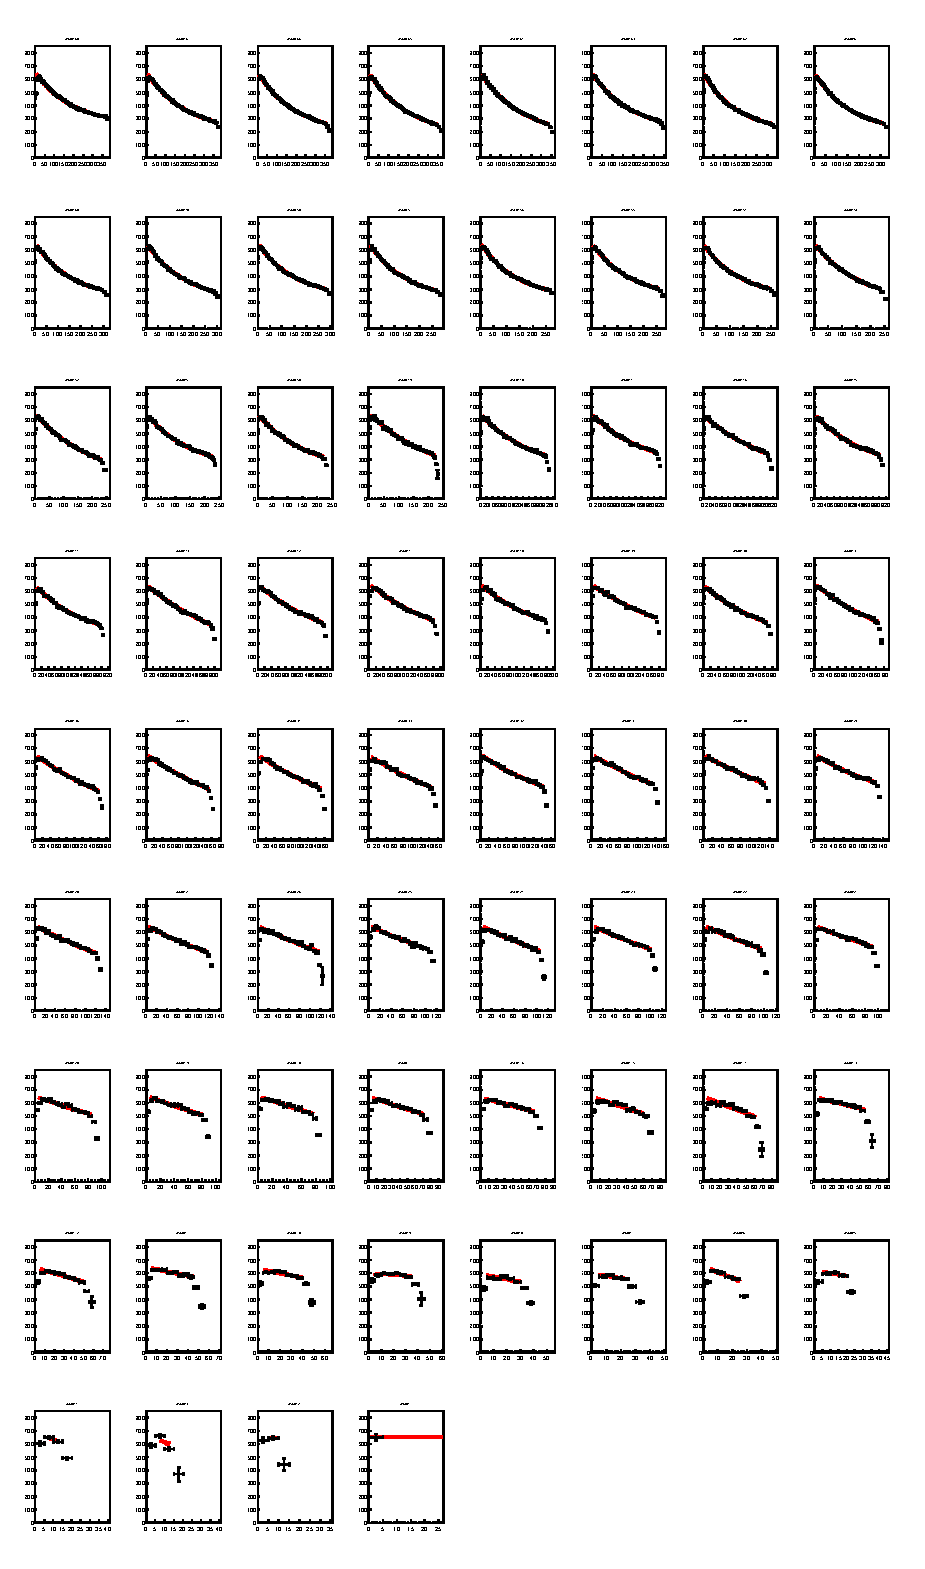
\includegraphics[width= 6.5in, height = 8in, keepaspectratio = true]{allustrips}
    \caption{Plotted are all of the u strip attenuation plots starting at 68 in the upper left hand corner. These plots are all plotted on a linear scale. The y-axis is set from 0 to 850 and the x-axis varies depending on the number of points in the plot.}
    \label{fig:allustrips}
\end{figure}

\FloatBarrier
%Vfits:
\begin{figure}[h]
    \centering
    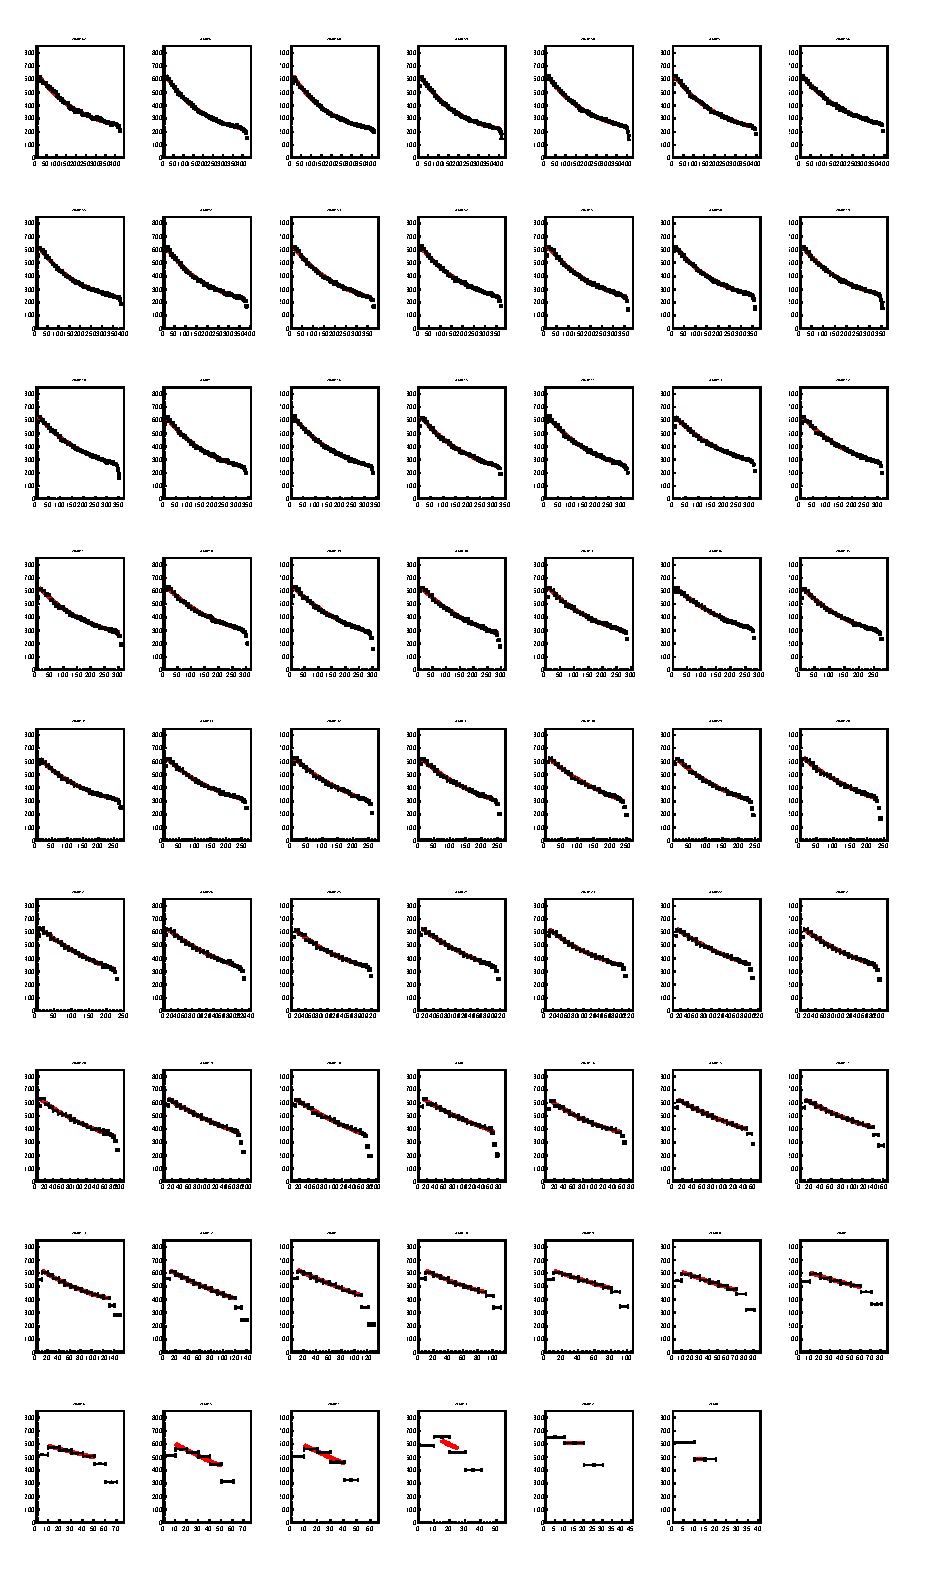
\includegraphics[width= 6.5in, height = 8in, keepaspectratio = true]{allvstrips}
    \caption{Plotted are all of the v strip attenuation plots starting at 62 in the upper left hand corner. These plots are all plotted on a linear scale. The y-axis is set from 0 to 850 and the x-axis varies depending on the number of points in the plot.}
    \label{fig:allvstrips}
\end{figure}


\FloatBarrier

%Wfits:
\begin{figure}[h]
    \centering
    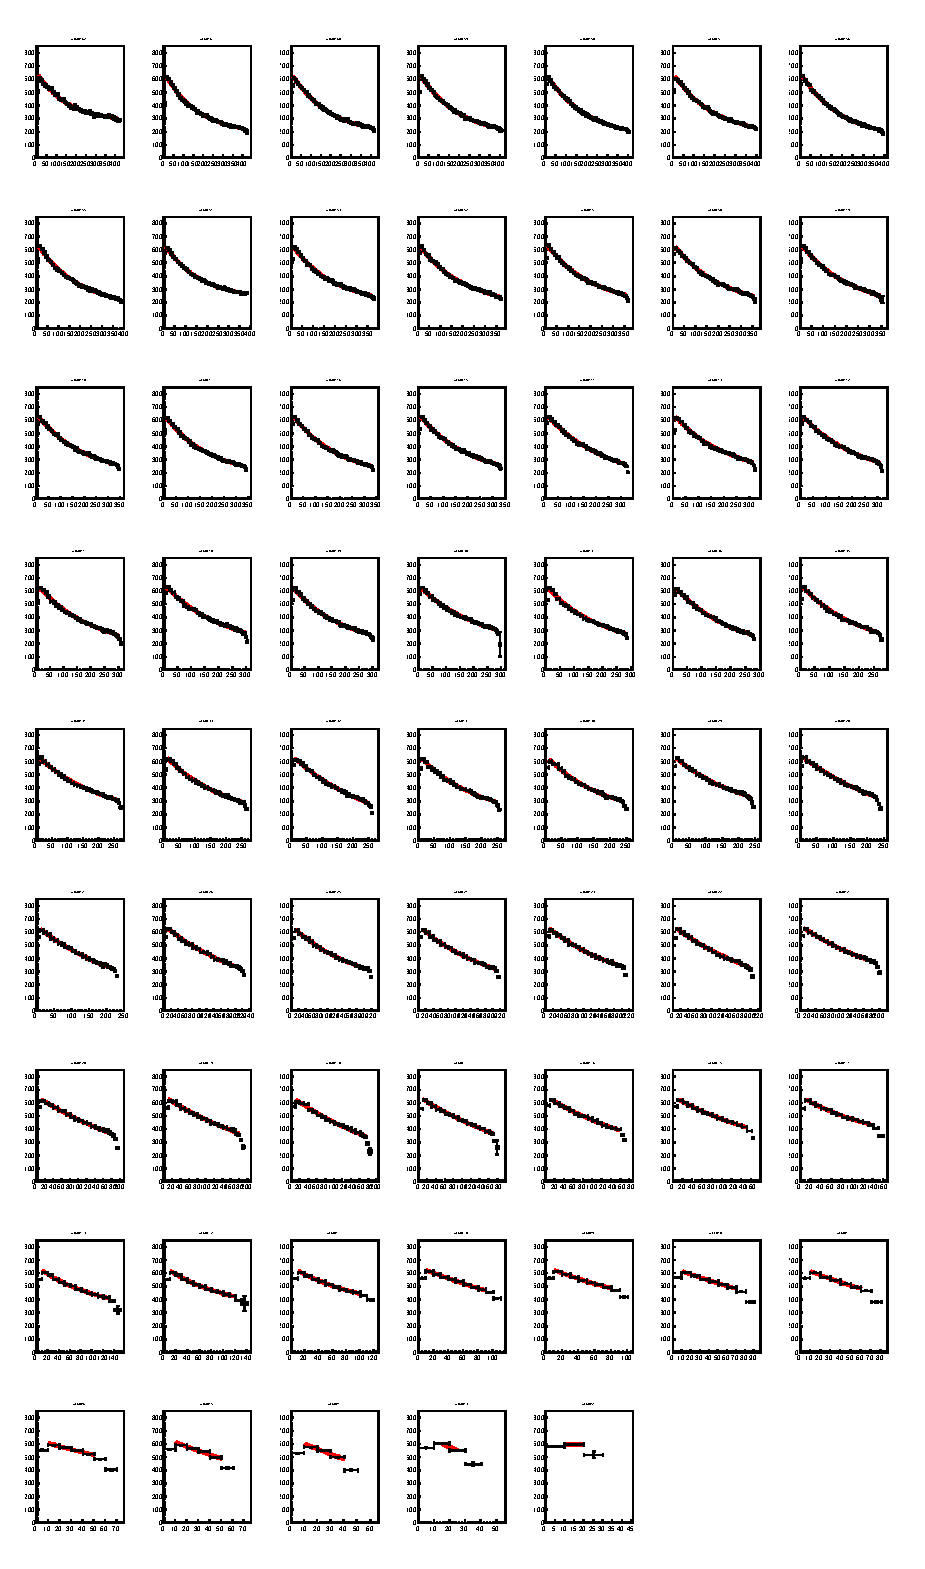
\includegraphics[width= 6.5in, height = 8in, keepaspectratio = true]{allwstrips}
    \caption{Plotted are all of the w strip attenuation plots starting at 62 in the upper left hand corner. These plots are all plotted on a linear scale. The y-axis is set from 0 to 850 and the x-axis varies depending on the number of points in the plot.}
    \label{fig:allustrips}
\end{figure}

\FloatBarrier
\begin{table}[h]
        \centering{}
        \scalebox{0.75}{
        \begin{tabular}{|c|c|c|c|}
            \hline
            U-Strip &  Parameter $a$  &Parameter $b$  & Parameter $c$ \\ \hline
1   &   650   &   0   &   0  \\  \hline  
2   &   650   &   0   &   0  \\  \hline  
3   &   650   &   -0.009   &   0  \\  \hline  
4   &   650   &   -0.009   &   0  \\  \hline  
5   &   616.113   &   -0.00639717   &   33.8858  \\  \hline  
6   &   649.996   &   -0.00717551   &   0.0046356  \\  \hline  
7   &   649.968   &   -0.00318808   &   0.0319326  \\  \hline  
8   &   649.972   &   -0.00232476   &   0.0273016  \\  \hline  
9   &   649.146   &   -0.00112904   &   0.854413  \\  \hline  
10   &   649.999   &   -0.00281005   &   0.000286188  \\  \hline  
11   &   649.993   &   -0.00286292   &   0.00718601  \\  \hline  
12   &   650   &   -0.0041656   &   0.000445736  \\  \hline  
13   &   650   &   -0.003283   &   0.000103724  \\  \hline  
14   &   649.997   &   -0.00376077   &   5.37227e-06  \\  \hline  
15   &   650.001   &   -0.00339912   &   6.96689e-06  \\  \hline  
16   &   649.997   &   -0.00305411   &   8.14649e-06  \\  \hline  
17   &   649.999   &   -0.00345134   &   9.95183e-09  \\  \hline  
18   &   649.998   &   -0.00310718   &   4.19396e-07  \\  \hline  
19   &   650   &   -0.00311517   &   5.01049e-06  \\  \hline  
20   &   650   &   -0.00281725   &   6.09084e-06  \\  \hline  
21   &   650   &   -0.00315783   &   3.38135e-05  \\  \hline  
22   &   650   &   -0.00328681   &   2.55834e-08  \\  \hline  
23   &   650   &   -0.00316776   &   2.15877e-05  \\  \hline  
24   &   649.999   &   -0.00317021   &   4.66803e-05  \\  \hline  
25   &   650   &   -0.00327065   &   5.9556e-06  \\  \hline  
26   &   650.001   &   -0.00309179   &   1.40689e-08  \\  \hline  
27   &   551.087   &   -0.00385902   &   98.9141  \\  \hline  
28   &   649.997   &   -0.00307714   &   7.49416e-05  \\  \hline  
29   &   419.522   &   -0.00552754   &   230.477  \\  \hline  
30   &   650   &   -0.00316014   &   0.000130702  \\  \hline  
31   &   650.001   &   -0.00312815   &   2.25921e-06  \\  \hline  
32   &   585.658   &   -0.00373922   &   64.3455  \\  \hline  
33   &   581.001   &   -0.00374214   &   68.997  \\  \hline  
34   &   650.002   &   -0.00328878   &   0.000131253  \\  \hline  
35   &   650   &   -0.00332314   &   1.43305e-05  \\  \hline  
36   &   649.998   &   -0.00340294   &   1.07435e-07  \\  \hline  
37   &   556.399   &   -0.00428136   &   93.5991  \\  \hline  
38   &   483.854   &   -0.00534903   &   166.146  \\  \hline  
39   &   482.458   &   -0.00431684   &   167.541  \\  \hline  
40   &   392.765   &   -0.00669036   &   257.235  \\  \hline  
41   &   499.22   &   -0.00443664   &   150.78  \\  \hline  
42   &   513.839   &   -0.00445738   &   136.164  \\  \hline  
43   &   581.507   &   -0.00388427   &   68.4914  \\  \hline  
44   &   391.463   &   -0.00757633   &   258.536  \\  \hline  
45   &   434.393   &   -0.00632194   &   215.608  \\  \hline  
46   &   463.813   &   -0.00513914   &   186.187  \\  \hline  
47   &   413.809   &   -0.00605594   &   236.189  \\  \hline  
48   &   442.234   &   -0.00592955   &   207.766  \\  \hline  
49   &   509.976   &   -0.00449146   &   140.024  \\  \hline  
50   &   443.895   &   -0.00614484   &   206.105  \\  \hline  
51   &   425.765   &   -0.00641114   &   224.233  \\  \hline  
52   &   504.812   &   -0.00511618   &   145.188  \\  \hline  
53   &   454.838   &   -0.0061679   &   195.162  \\  \hline  
54   &   406.411   &   -0.00766326   &   243.589  \\  \hline  
55   &   415.976   &   -0.00690821   &   234.026  \\  \hline  
56   &   421.326   &   -0.00710769   &   228.675  \\  \hline  
57   &   435.635   &   -0.00660386   &   214.362  \\  \hline  
58   &   411.518   &   -0.00663318   &   238.483  \\  \hline  
59   &   438.882   &   -0.00625669   &   211.118  \\  \hline  
60   &   423.763   &   -0.00618908   &   226.238  \\  \hline  
61   &   444.671   &   -0.0063621   &   205.328  \\  \hline  
62   &   438.481   &   -0.00674885   &   211.519  \\  \hline  
63   &   437.138   &   -0.00564978   &   212.862  \\  \hline  
64   &   482.525   &   -0.00495599   &   167.473  \\  \hline  
65   &   473.388   &   -0.00516614   &   176.613  \\  \hline  
66   &   465.633   &   -0.00500512   &   184.367  \\  \hline  
67   &   455.941   &   -0.00479029   &   194.059  \\  \hline  
68   &   410.201   &   -0.00506009   &   239.798  \\  \hline  
        \end{tabular}
        }
        \caption{Calibration Constants for the U layer.}
\end{table}


\begin{table}[h]
        \centering
        \scalebox{0.75}{
        \begin{tabular}{|c|c|c|c|}
            \hline
            V-Strip &  Parameter $a$  &Parameter $b$  & Parameter $c$ \\ \hline
1   &   650.002   &   0   &   0  \\  \hline  
2   &   649.999   &   0   &   0  \\  \hline  
3   &   650.001   &   -0.009   &   0  \\  \hline  
4   &   650.001   &   -0.009   &   8.41036e-07  \\  \hline  
5   &   650   &   -0.00794645   &   5.04738e-06  \\  \hline  
6   &   649.225   &   -0.00402729   &   0.773706  \\  \hline  
7   &   341.165   &   -0.009   &   308.835  \\  \hline  
8   &   649.999   &   -0.0043402   &   0.000921065  \\  \hline  
9   &   650   &   -0.00346629   &   0.00030414  \\  \hline  
10   &   409.661   &   -0.0073313   &   240.338  \\  \hline  
11   &   650   &   -0.0036951   &   0.000157707  \\  \hline  
12   &   543.255   &   -0.00487653   &   106.745  \\  \hline  
13   &   385.429   &   -0.00755387   &   264.571  \\  \hline  
14   &   462.536   &   -0.00523798   &   187.463  \\  \hline  
15   &   490.318   &   -0.00478212   &   159.682  \\  \hline  
16   &   409.407   &   -0.00682511   &   240.592  \\  \hline  
17   &   644.496   &   -0.00311038   &   5.50402  \\  \hline  
18   &   649.997   &   -0.00345834   &   1.60129e-06  \\  \hline  
19   &   650   &   -0.00314254   &   4.40293e-06  \\  \hline  
20   &   476.84   &   -0.00525174   &   173.161  \\  \hline  
21   &   504.696   &   -0.00482932   &   145.304  \\  \hline  
22   &   501.641   &   -0.00447931   &   148.359  \\  \hline  
23   &   427.011   &   -0.00618067   &   222.989  \\  \hline  
24   &   532.597   &   -0.00429752   &   117.404  \\  \hline  
25   &   452.731   &   -0.00555935   &   197.267  \\  \hline  
26   &   514.63   &   -0.00444436   &   135.371  \\  \hline  
27   &   562.158   &   -0.00411837   &   87.8438  \\  \hline  
28   &   552.525   &   -0.00397784   &   97.4754  \\  \hline  
29   &   505.009   &   -0.00490977   &   144.992  \\  \hline  
30   &   545.684   &   -0.00417772   &   104.316  \\  \hline  
31   &   520.37   &   -0.00441109   &   129.628  \\  \hline  
32   &   545.125   &   -0.00412529   &   104.875  \\  \hline  
33   &   454.001   &   -0.00531295   &   195.999  \\  \hline  
34   &   430.052   &   -0.00591867   &   219.949  \\  \hline  
35   &   472.603   &   -0.00523221   &   177.394  \\  \hline  
36   &   479.173   &   -0.0044464   &   170.826  \\  \hline  
37   &   472.073   &   -0.00500161   &   177.926  \\  \hline  
38   &   521.65   &   -0.00433543   &   128.35  \\  \hline  
39   &   523.67   &   -0.00413843   &   126.33  \\  \hline  
40   &   475.448   &   -0.00450584   &   174.551  \\  \hline  
41   &   463.401   &   -0.0051012   &   186.6  \\  \hline  
42   &   486.03   &   -0.0046867   &   163.97  \\  \hline  
43   &   474.905   &   -0.00454652   &   175.094  \\  \hline  
44   &   512.336   &   -0.00460079   &   137.664  \\  \hline  
45   &   518.211   &   -0.00460405   &   131.79  \\  \hline  
46   &   503.032   &   -0.00487218   &   146.968  \\  \hline  
47   &   501.666   &   -0.00500745   &   148.335  \\  \hline  
48   &   488.139   &   -0.00450074   &   161.861  \\  \hline  
49   &   479.791   &   -0.00489837   &   170.209  \\  \hline  
50   &   487.47   &   -0.00479649   &   162.531  \\  \hline  
51   &   516.592   &   -0.0043148   &   133.409  \\  \hline  
52   &   504.835   &   -0.0045441   &   145.166  \\  \hline  
53   &   516.386   &   -0.00442848   &   133.615  \\  \hline  
54   &   493.162   &   -0.0051403   &   156.838  \\  \hline  
55   &   475.544   &   -0.00530062   &   174.455  \\  \hline  
56   &   483.85   &   -0.00428974   &   166.15  \\  \hline  
57   &   493.428   &   -0.00469419   &   156.572  \\  \hline  
58   &   485.197   &   -0.00470872   &   164.802  \\  \hline  
59   &   484.814   &   -0.00529538   &   165.185  \\  \hline  
60   &   492.715   &   -0.00499336   &   157.285  \\  \hline  
61   &   496.221   &   -0.00497787   &   153.779  \\  \hline  
62   &   472.264   &   -0.00469273   &   177.736  \\  \hline    
        \end{tabular}
        }
        \caption{Calibration Constants for the V layer.}
\end{table}


\begin{table}[h]
        \centering
        \scalebox{0.75}{
        \begin{tabular}{|c|c|c|c|}
            \hline
            W-Strip &  Parameter $a$  &Parameter $b$  & Parameter $c$ \\ \hline
1   &   650   &   0   &   0  \\  \hline  
0   &   650   &   0   &   0  \\  \hline  
0   &   650   &   -0.009   &   0  \\  \hline  
0   &   649.996   &   -0.00691378   &   0.00571745  \\  \hline  
0   &   650   &   -0.00558302   &   0.000738429  \\  \hline  
0   &   649.98   &   -0.00407219   &   0.0177906  \\  \hline  
0   &   422.924   &   -0.0082021   &   227.077  \\  \hline  
0   &   505.741   &   -0.00555023   &   144.259  \\  \hline  
0   &   372.286   &   -0.00737429   &   277.714  \\  \hline  
0   &   649.979   &   -0.00366028   &   0.0192191  \\  \hline  
0   &   650.001   &   -0.00372954   &   0.00118075  \\  \hline  
0   &   342.164   &   -0.009   &   307.836  \\  \hline  
0   &   355.773   &   -0.00855197   &   294.227  \\  \hline  
0   &   363.361   &   -0.00666561   &   286.64  \\  \hline  
0   &   434.311   &   -0.00525056   &   215.689  \\  \hline  
0   &   556.671   &   -0.00394053   &   93.3294  \\  \hline  
0   &   649.998   &   -0.00335208   &   7.53184e-06  \\  \hline  
0   &   650.001   &   -0.00360869   &   0.000280125  \\  \hline  
0   &   650   &   -0.00315057   &   1.4947e-05  \\  \hline  
0   &   650   &   -0.00319373   &   1.11969e-05  \\  \hline  
0   &   527.95   &   -0.00400632   &   122.05  \\  \hline  
0   &   618.622   &   -0.00362112   &   31.3758  \\  \hline  
0   &   500.057   &   -0.00478853   &   149.941  \\  \hline  
0   &   548.15   &   -0.00446747   &   101.85  \\  \hline  
0   &   479.19   &   -0.00563269   &   170.81  \\  \hline  
0   &   577.911   &   -0.00381978   &   72.0904  \\  \hline  
0   &   571.915   &   -0.00386651   &   78.0872  \\  \hline  
0   &   650   &   -0.00301759   &   6.97793e-06  \\  \hline  
0   &   476.296   &   -0.00466684   &   173.704  \\  \hline  
0   &   469.596   &   -0.0056956   &   180.406  \\  \hline  
0   &   483.094   &   -0.00545448   &   166.906  \\  \hline  
0   &   648.632   &   -0.0033354   &   1.3664  \\  \hline  
0   &   496.17   &   -0.00515118   &   153.83  \\  \hline  
0   &   487.383   &   -0.00461829   &   162.617  \\  \hline  
0   &   506.497   &   -0.00489625   &   143.503  \\  \hline  
0   &   517.17   &   -0.00494086   &   132.832  \\  \hline  
0   &   464.957   &   -0.00562927   &   185.046  \\  \hline  
0   &   481.521   &   -0.00435674   &   168.479  \\  \hline  
0   &   461.989   &   -0.00582562   &   188.011  \\  \hline  
0   &   499.489   &   -0.00442904   &   150.51  \\  \hline  
0   &   506.749   &   -0.00475107   &   143.248  \\  \hline  
0   &   502.841   &   -0.00434983   &   147.157  \\  \hline  
0   &   469.808   &   -0.00484038   &   180.192  \\  \hline  
0   &   527.099   &   -0.00412014   &   122.901  \\  \hline  
0   &   486.457   &   -0.00490661   &   163.543  \\  \hline  
0   &   489.691   &   -0.00510504   &   160.309  \\  \hline  
0   &   471.254   &   -0.00553953   &   178.746  \\  \hline  
0   &   472.808   &   -0.0050091   &   177.192  \\  \hline  
0   &   509.753   &   -0.00440386   &   140.247  \\  \hline  
0   &   487.851   &   -0.00484449   &   162.148  \\  \hline  
0   &   484.151   &   -0.0047396   &   165.851  \\  \hline  
0   &   479.294   &   -0.00498712   &   170.706  \\  \hline  
0   &   468.169   &   -0.00519666   &   181.83  \\  \hline  
0   &   427.693   &   -0.00598915   &   222.306  \\  \hline  
0   &   491.659   &   -0.00526729   &   158.341  \\  \hline  
0   &   514.732   &   -0.0050567   &   135.269  \\  \hline  
0   &   475.716   &   -0.00527028   &   174.285  \\  \hline  
0   &   500.373   &   -0.00518313   &   149.628  \\  \hline  
0   &   496.167   &   -0.00495883   &   153.833  \\  \hline  
0   &   475.153   &   -0.00531751   &   174.847  \\  \hline  
0   &   476.541   &   -0.00557183   &   173.458  \\  \hline  
0   &   371.958   &   -0.00688108   &   278.043  \\  \hline   
        \end{tabular}
        }
        \caption{Calibration Constants for the W layer.}
\end{table}


\FloatBarrier
\begin{table}[h]
    \begin{subtable}[h]{2in}
        \centering{}
        \scalebox{.7}{
        \begin{tabular}{|c|c|}
            \hline
            U-Strip & Gain\\ \hline
68   &   0.919826  \\  \hline  
67   &   0.994387  \\  \hline  
66   &   0.996668  \\  \hline  
65   &   1.13365  \\  \hline  
64   &   1.0289  \\  \hline  
63   &   0.988108  \\  \hline  
62   &   1.05729  \\  \hline  
61   &   1.00024  \\  \hline  
60   &   0.918702  \\  \hline  
59   &   0.937388  \\  \hline  
58   &   0.971579  \\  \hline  
57   &   0.968278  \\  \hline  
56   &   0.9886  \\  \hline  
55   &   1.01584  \\  \hline  
54   &   0.972431  \\  \hline  
53   &   0.985789  \\  \hline  
52   &   1.06724  \\  \hline  
51   &   1.06537  \\  \hline  
50   &   1.15373  \\  \hline  
49   &   1.05132  \\  \hline  
48   &   1.05095  \\  \hline  
47   &   0.990354  \\  \hline  
46   &   1.05387  \\  \hline  
45   &   1.00345  \\  \hline  
44   &   0.90308  \\  \hline  
43   &   1.05416  \\  \hline  
42   &   1.03789  \\  \hline  
41   &   1.08503  \\  \hline  
40   &   0.964149  \\  \hline  
39   &   0.984689  \\  \hline  
38   &   1.07509  \\  \hline  
37   &   1.02063  \\  \hline  
36   &   0.973037  \\  \hline  
35   &   0.960093  \\  \hline  
34   &   0.999216  \\  \hline  
33   &   1.01442  \\  \hline  
32   &   0.966014  \\  \hline  
31   &   1.01264  \\  \hline  
30   &   1.01884  \\  \hline  
29   &   0.99361  \\  \hline  
28   &   1.12513  \\  \hline  
27   &   1.11908  \\  \hline  
26   &   1.14991  \\  \hline  
25   &   0.99626  \\  \hline  
24   &   1.01688  \\  \hline  
23   &   1.04101  \\  \hline  
22   &   0.993246  \\  \hline  
21   &   1.00052  \\  \hline  
20   &   0.927249  \\  \hline  
19   &   0.943803  \\  \hline  
18   &   0.975746  \\  \hline  
17   &   1.0319  \\  \hline  
16   &   1.05238  \\  \hline  
15   &   1.03268  \\  \hline  
14   &   0.999323  \\  \hline  
13   &   1.07013  \\  \hline  
12   &   0.974823  \\  \hline  
11   &   1.02237  \\  \hline  
10   &   1.0473  \\  \hline  
9   &   1.00103  \\  \hline  
8   &   1.13001  \\  \hline  
7   &   0.979758  \\  \hline  
6   &   0.945828  \\  \hline  
5   &   1.06426  \\  \hline  
4   &   1.08689  \\  \hline  
3   &   1.00753  \\  \hline  
2   &   1.03341  \\  \hline  
1   &   2.38937  \\  \hline   
        \end{tabular}
        }
        \caption{Gains for the U layer.}
    \end{subtable}
    \quad
    \begin{subtable}[h]{2in}
        \centering{}
        \scalebox{.7}{
        \begin{tabular}{|c|c|}
            \hline
            V-Strip & Gain \\ \hline
62   &   0.856903  \\  \hline  
61   &   0.975891  \\  \hline  
60   &   0.957263  \\  \hline  
59   &   0.984709  \\  \hline  
58   &   0.945978  \\  \hline  
57   &   0.94414  \\  \hline  
56   &   0.929243  \\  \hline  
55   &   0.981845  \\  \hline  
54   &   1.00783  \\  \hline  
53   &   0.970635  \\  \hline  
52   &   0.99664  \\  \hline  
51   &   0.984337  \\  \hline  
50   &   0.9841  \\  \hline  
49   &   1.02766  \\  \hline  
48   &   0.972439  \\  \hline  
47   &   1.05155  \\  \hline  
46   &   1.03861  \\  \hline  
45   &   0.98368  \\  \hline  
44   &   1.00809  \\  \hline  
43   &   0.991325  \\  \hline  
42   &   0.989896  \\  \hline  
41   &   0.965113  \\  \hline  
40   &   0.939102  \\  \hline  
39   &   1.05284  \\  \hline  
38   &   1.04087  \\  \hline  
37   &   0.972662  \\  \hline  
36   &   0.980653  \\  \hline  
35   &   0.993551  \\  \hline  
34   &   0.961802  \\  \hline  
33   &   1.01387  \\  \hline  
32   &   1.03706  \\  \hline  
31   &   1.04414  \\  \hline  
30   &   1.00396  \\  \hline  
29   &   0.994342  \\  \hline  
28   &   0.993199  \\  \hline  
27   &   1.00151  \\  \hline  
26   &   1.04742  \\  \hline  
25   &   1.05564  \\  \hline  
24   &   1.08135  \\  \hline  
23   &   0.971184  \\  \hline  
22   &   0.916638  \\  \hline  
21   &   1.026  \\  \hline  
20   &   0.978999  \\  \hline  
19   &   1.0785  \\  \hline  
18   &   1.03334  \\  \hline  
17   &   1.00605  \\  \hline  
16   &   1.02326  \\  \hline  
15   &   0.947529  \\  \hline  
14   &   0.943325  \\  \hline  
13   &   0.978369  \\  \hline  
12   &   0.965212  \\  \hline  
11   &   0.94848  \\  \hline  
10   &   1.05385  \\  \hline  
9   &   0.960673  \\  \hline  
8   &   1.04593  \\  \hline  
7   &   0.965207  \\  \hline  
6   &   0.930664  \\  \hline  
5   &   0.924364  \\  \hline  
4   &   0.906707  \\  \hline  
3   &   0.994952  \\  \hline  
2   &   1.11947  \\  \hline  
1   &   1.16553  \\  \hline  
        \end{tabular}
        }
        \caption{Gains for the V layer.}
    \end{subtable}
    \quad
    \begin{subtable}[h]{2in}
        \centering{}
        \scalebox{0.7}{
        \begin{tabular}{|c|c|}
            \hline
            W-Strip & Gain  \\ \hline
62   &   0.984625  \\  \hline  
61   &   1.04515  \\  \hline  
60   &   0.984452  \\  \hline  
59   &   1.05211  \\  \hline  
58   &   1.01464  \\  \hline  
57   &   1.01152  \\  \hline  
56   &   1.12032  \\  \hline  
55   &   1.08628  \\  \hline  
54   &   1.04743  \\  \hline  
53   &   1.03443  \\  \hline  
52   &   0.973068  \\  \hline  
51   &   0.986971  \\  \hline  
50   &   1.0584  \\  \hline  
49   &   1.02468  \\  \hline  
48   &   1.00968  \\  \hline  
47   &   1.03928  \\  \hline  
46   &   1.1033  \\  \hline  
45   &   1.00978  \\  \hline  
44   &   1.01194  \\  \hline  
43   &   0.991657  \\  \hline  
42   &   1.04533  \\  \hline  
41   &   1.07685  \\  \hline  
40   &   1.0462  \\  \hline  
39   &   1.01952  \\  \hline  
38   &   1.04494  \\  \hline  
37   &   0.940542  \\  \hline  
36   &   1.07141  \\  \hline  
35   &   1.02338  \\  \hline  
34   &   1.01296  \\  \hline  
33   &   0.977284  \\  \hline  
32   &   1.11503  \\  \hline  
31   &   0.955289  \\  \hline  
30   &   1.00997  \\  \hline  
29   &   0.980596  \\  \hline  
28   &   0.999784  \\  \hline  
27   &   1.0662  \\  \hline  
26   &   1.01917  \\  \hline  
25   &   0.998049  \\  \hline  
24   &   1.07542  \\  \hline  
23   &   1.01097  \\  \hline  
22   &   1.00608  \\  \hline  
21   &   0.995989  \\  \hline  
20   &   1.00445  \\  \hline  
19   &   1.04812  \\  \hline  
18   &   1.05886  \\  \hline  
17   &   1.00316  \\  \hline  
16   &   1.00583  \\  \hline  
15   &   0.920611  \\  \hline  
14   &   0.95728  \\  \hline  
13   &   0.928774  \\  \hline  
12   &   0.932801  \\  \hline  
11   &   0.975309  \\  \hline  
10   &   1.02923  \\  \hline  
9   &   0.969189  \\  \hline  
8   &   0.978204  \\  \hline  
7   &   0.927413  \\  \hline  
6   &   1.01355  \\  \hline  
5   &   1.00309  \\  \hline  
4   &   0.965665  \\  \hline  
3   &   0.959464  \\  \hline  
2   &   1.1257  \\  \hline  
1   &   1  \\  \hline  
        \end{tabular}
        }
        \caption{Gains for the W layer.}
    \end{subtable}
    \caption{Preliminary Gains}
\end{table}








\section{Calibration Studies}

\FloatBarrier
\subsection{Optimal ADC Bin Size}
\label{sec:OptimalBin}
A study was performed to view an optimal binning of the ADC readout. 
The ADC readout was plotted from zero to one thousand. 
This study looked at the effect from variation of the number of bins. 
The final Gaussian fit was used on each signal pixel when finding differences. 
It is clear that the optimal binsize is limited by the small pixel readouts, or the portion of the detector nearest the beam line. Therefore a reasonable limit on the smallest bin size (for these statistics) was estimated to be around $\frac{1000}{200}=5$ on the ADC readout. To get more trustworthy fits a choice was made of bin size to be $\frac{1000}{125}=8$ on the ADC readout.


\FloatBarrier
\subsection{Minimum Statistics}
A minor study was conducted to determine the minimum statistics needed for calibration of the PCAL unit.
However, this is tangled into multiple different components.
Adjusting the bin size might affect the total statistics needed.
This study only focuses on the optimal bin size determined by section \ref{sec:OptimalBin}.
Another factor for the amount of statistics needed is the physical bin size.
This limits the overall statisics to the lowest number needed to calibrate the shortest strips (i.e. low u strip number, high w/v strip number).
Figure \ref{fig:statstud1} shows the first few u-strips (strips 3 through 8), that are physically binned by the w-strips.

If these strips are to be calibrated and the ADC bin size is to stay the same, then based on these plots the minimum statistics needed is roughly equal to the data obtained currently.
This analysis contains 5.2 billion post-skimmed events.
This equilavates to a days worth of data with the PCAL unit laid out horizontally.
Due to the decrease of the cosmic ray flux when the unit is vertically aligned, a larger time scale will be needed.
\FloatBarrier{}


\begin{figure}
    \centering
    \begin{subfigure}[h]{0.4\textwidth}
        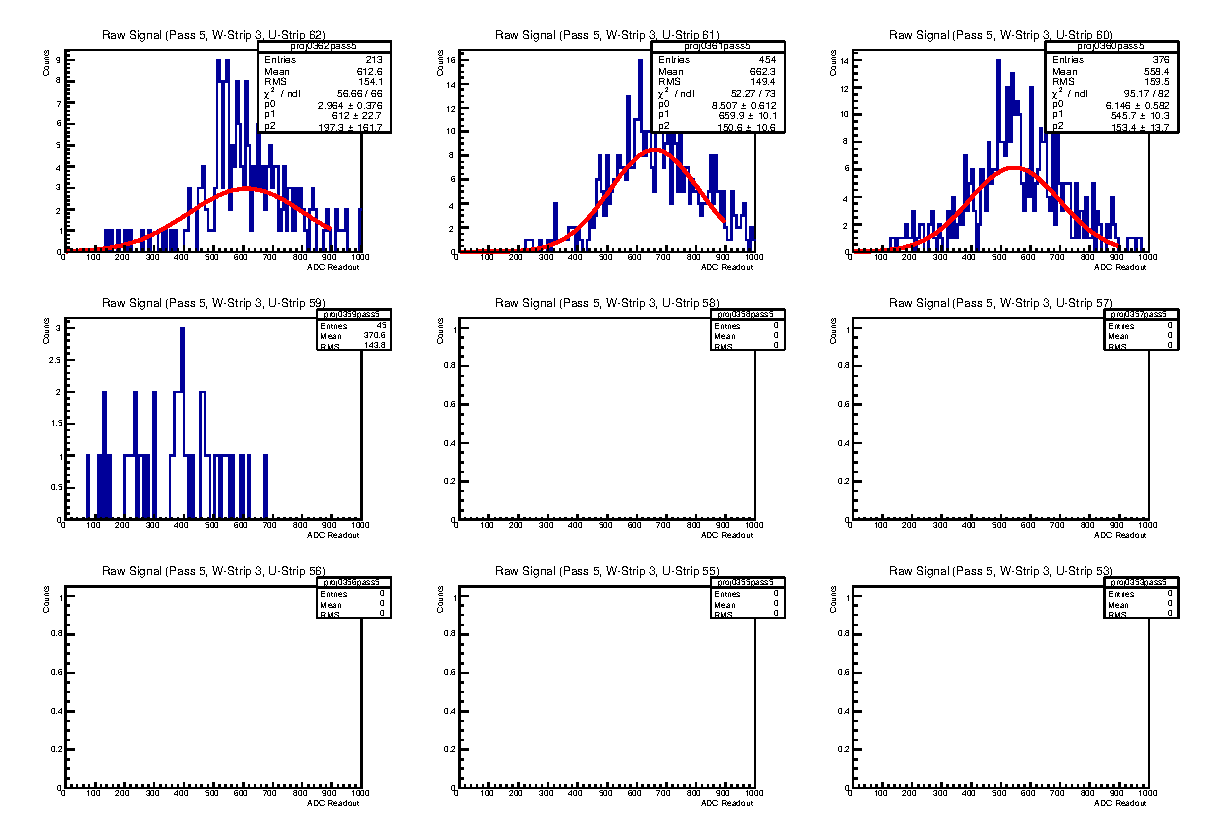
\includegraphics[width= \textwidth, keepaspectratio = true]{ustrip3}
        \caption{Shown are all of the w projections onto u-strip 3. The distribution shown peaks around 15 counts.}
        \label{fig:ustrip3}
    \end{subfigure}
    ~
    \begin{subfigure}[h]{0.4\textwidth}
        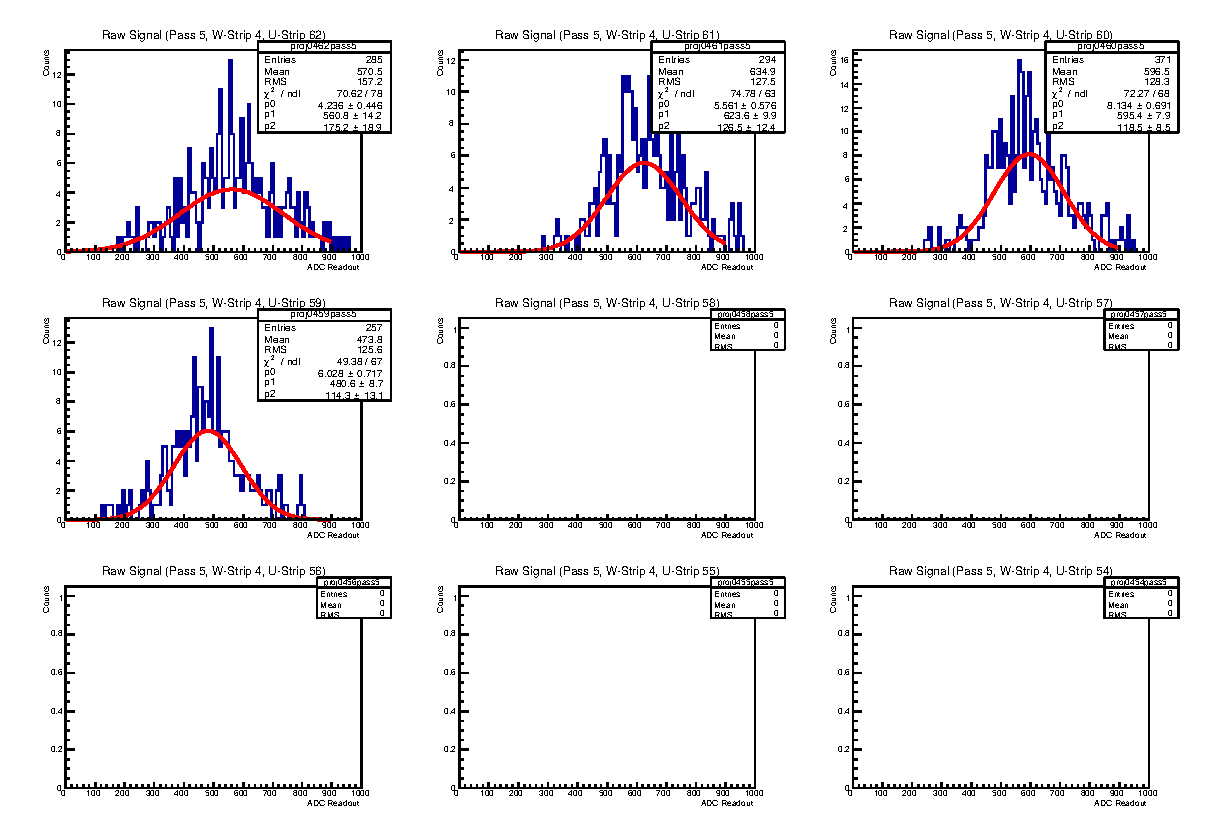
\includegraphics[width= \textwidth, keepaspectratio = true]{ustrip4}
        \caption{Shown are all of the w projections onto u-strip 4. The distribution shown peaks around 15 counts.}
        \label{fig:ustrip4}
    \end{subfigure}
    ~
    \begin{subfigure}[h]{0.4\textwidth}
        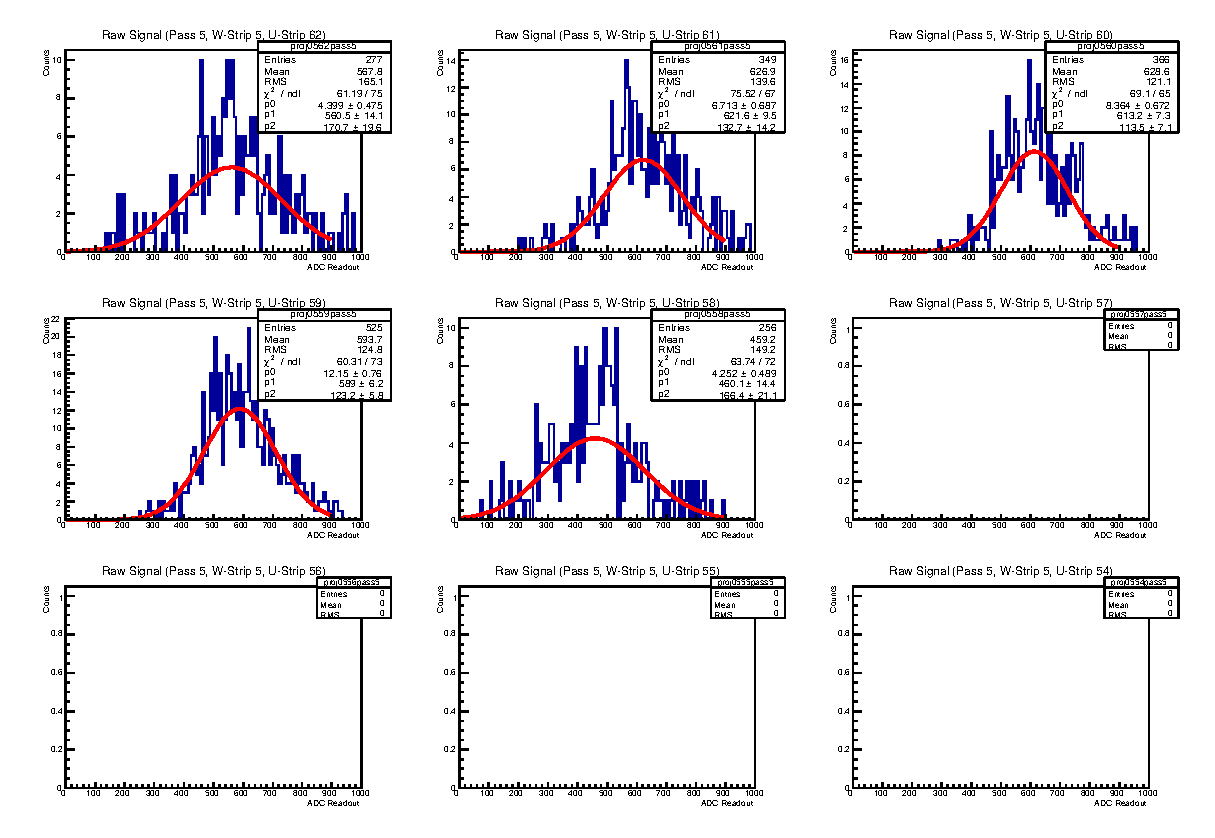
\includegraphics[width= \textwidth, keepaspectratio = true]{ustrip5}
        \caption{Shown are all of the w projections onto u-strip 5. The distribution shown peaks around 15 counts.}
        \label{fig:ustrip5}
    \end{subfigure}
    ~
    \begin{subfigure}[h]{0.4\textwidth}
        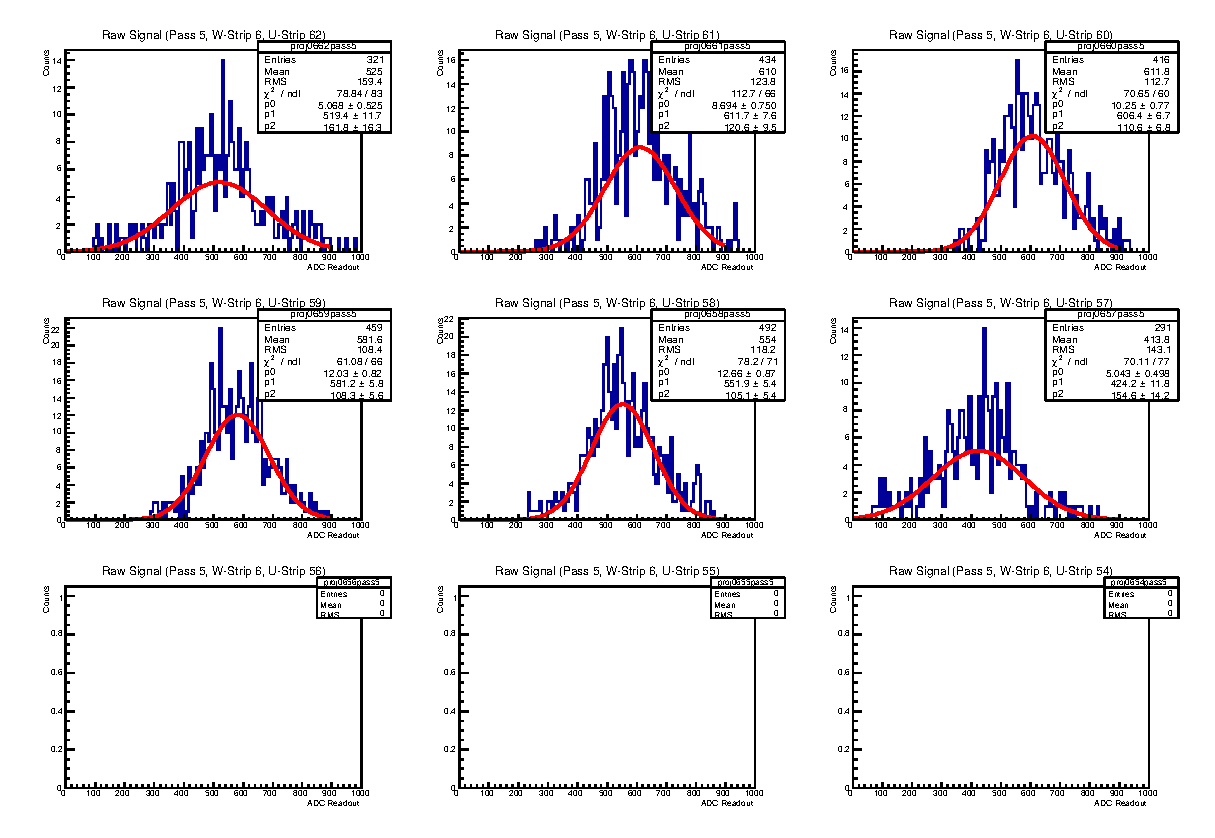
\includegraphics[width= \textwidth, keepaspectratio = true]{ustrip6}
        \caption{Shown are all of the w projections onto u-strip 6. The distribution shown peaks around 15 counts.}
        \label{fig:ustrip6}
    \end{subfigure}
    ~
    \begin{subfigure}[h]{0.4\textwidth}
        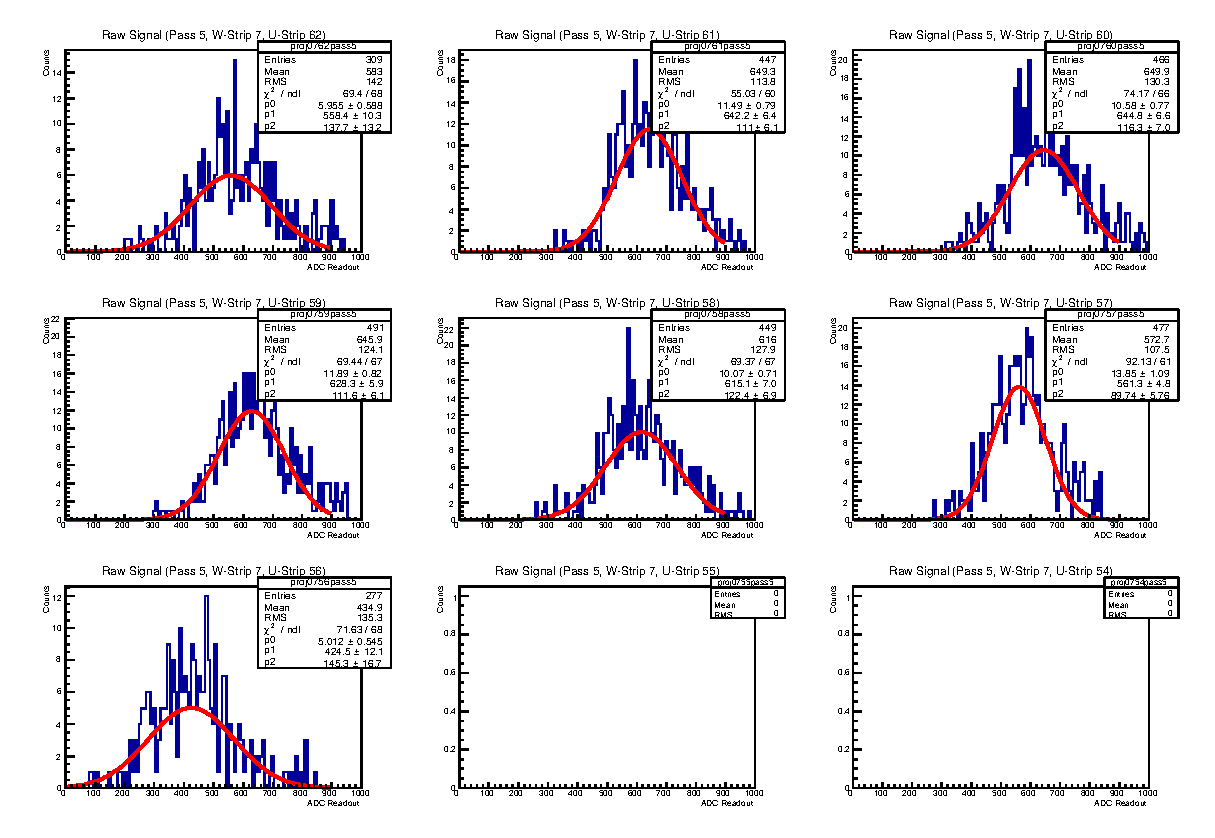
\includegraphics[width= \textwidth, keepaspectratio = true]{ustrip7}
        \caption{Shown are all of the w projections onto u-strip 7. The distribution shown peaks around 15 counts.}
        \label{fig:ustrip7}
    \end{subfigure}
    ~
    \begin{subfigure}[h]{0.4\textwidth}
        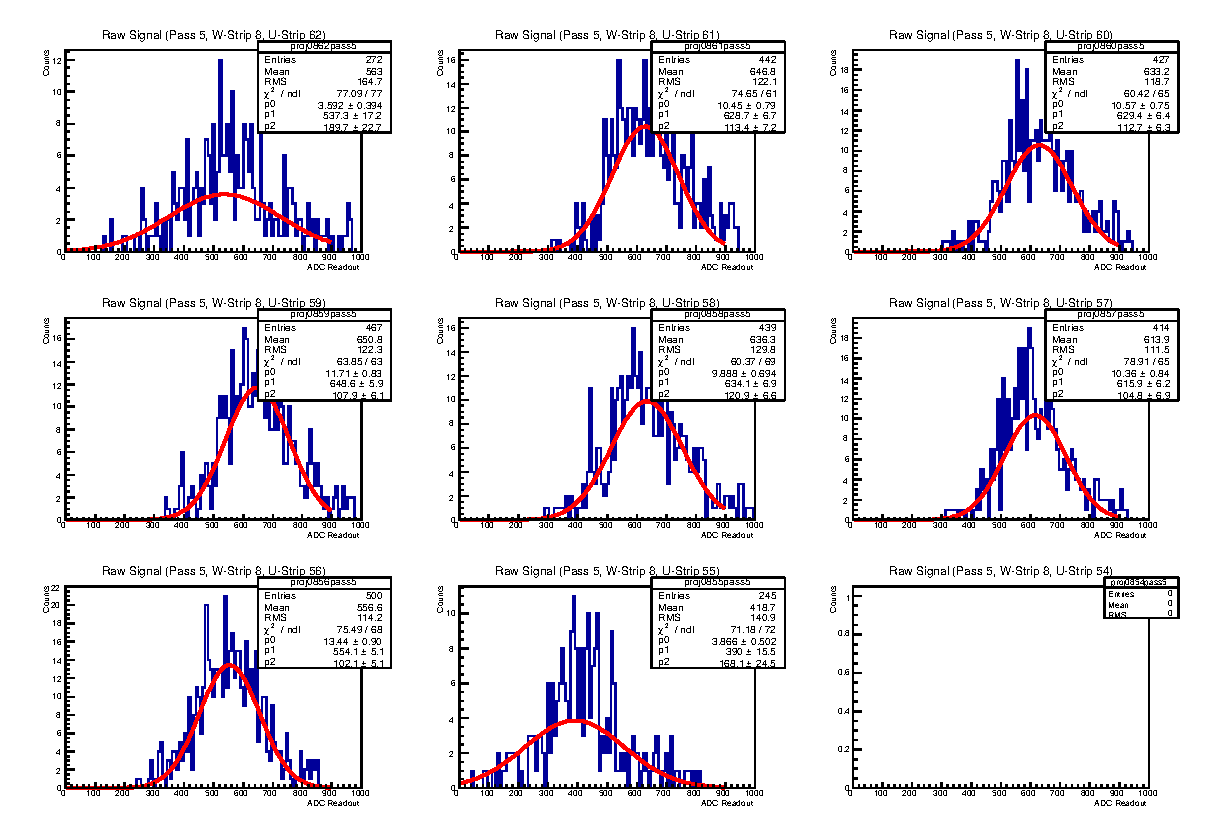
\includegraphics[width= \textwidth, keepaspectratio = true]{ustrip8}
        \caption{Shown are all of the w projections onto u-strip 8. The distribution shown peaks around 15 counts.}
        \label{fig:ustrip8}
    \end{subfigure}
    \caption{Plotted are a six of the short scintillator strips. Each subfigure shows projections of the last 9 w-strips. Therefore these plot axises are counts versus ADC value detected by the u layer PMT.}
    \label{fig:statstud1}
\end{figure}


\FloatBarrier


\begin{thebibliography}{99}
 
 \bibitem{bib:geomnote}
  G. Asryan et al.,
  \emph{\url{https://clasweb.jlab.org/wiki/images/d/d0/Pcal_geometry_note.pdf}}

   \bibitem{bib:cosmicweb}
  %C. Smith,
  \emph{\url{https://clasweb.jlab.org/wiki/index.php/PCAL_Cosmic_Ray_Tests}}


  
 
\end{thebibliography}




\end{document}
